%-------------------------------------------------------------------------
%-------------------------------------------------------------------------
%-------------------------------------------------------------------------

\chapter[Design Study\texorpdfstring{:\\ Matches, Mismatches, and Methods: Multiple-View Workflows for Energy Portfolio Analysis}{}]{Design Study\texorpdfstring{:\\ \large{Matches, Mismatches, and Methods: Multiple-View Workflows for Energy Portfolio Analysis}}{}}
\label{ch:emu}

%-------------------------------------------------------------------------
%-------------------------------------------------------------------------
%-------------------------------------------------------------------------

% \begin{epigraph}
%     \item (quote needed)
% \end{epigraph}

\footnote{This chapter is a slightly modified version of our paper {\it Matches, Mismatches, and Methods: Multiple-View Workflows for Energy Portfolio Analysis} by Matthew Brehmer, Jocelyn Ng, Kevin Tate, and Tamara Munzner; in IEEE Transactions on Visualization and Computer Graphics (Proceedings of InfoVis 2015), 22(1), p. 449--458~\cite{Brehmer2015}. \url{http://dx.doi.org/10.1109/TVCG.2015.2466971}. \autoref{emu:addendum} is a new addendum section that is unique to this dissertation.}The energy performance of large building portfolios is challenging to analyze and monitor, as current analysis tools are not scalable or they present derived and aggregated data at too coarse of a level. 
We conducted a visualization design study\index{design studies}, beginning with a thorough work domain analysis\index{work domain analysis} and a classification of data\index{data abstraction} and task abstractions\index{task!task abstraction}. 
We describe visual encoding\index{visual encoding} design choices for time-oriented data\index{time-oriented data} framed in terms of {\it matches} and {\it mismatches}, as well as considerations for workflow design\index{workflows!workflow design}. 
Our designs address several research questions pertaining to scalability, view coordination\index{view coordination}, and the inappropriateness of line graphs\index{visual encoding!line graph} for derived\index{{\tt derive}} and aggregated\index{{\tt aggregate}} data. 
We also present guidelines relating to {\it familiarity}\index{familiarity} and {\it trust}, as well as methodological considerations for visualization design studies\index{design studies}. 
Our designs were adopted\index{adoption} by our collaborators and incorporated into the design of an energy analysis software application that will be deployed to their large client base.

%-------------------------------------------------------------------------
%-------------------------------------------------------------------------

\section{Motivation}
\label{emu:introduction}

%-------------------------------------------------------------------------
%-------------------------------------------------------------------------

Consider a university campus containing about a hundred buildings. 
For a university operations worker looking for opportunities to conserve energy, visualization can be helpful when analyzing and monitoring the energy performance of this large portfolio of buildings. 

In this design study\index{design studies}, we collaborated with a team of people at EnerNOC, a company that develops energy analysis and reporting software for organizations such as commercial business chains, universities, and utility companies.
Our collaborators' goal was to deploy a redesigned version of Energy Manager\index{Energy Manager}, their energy analysis software tool; in doing so, they hoped to retain their existing client base encompassing thousands of organizations, attract new clients, and increase engagement with their software. 
Meanwhile, our goal as researchers was to successfully integrate our research process into our collaborators' software development practice.
We designed and evaluated\index{evaluation} potential visual encodings\index{visual encoding} and interactions\index{interaction} with a variety of stakeholders in an industry setting, which included our collaborators' colleagues as well as their clients.
This chapter documents a success story, where our collaborators committed software development resources and adopted\index{adoption} our designs that resulted from our research.

Visualization researchers and practitioners working in domains unrelated to energy analysis will find several transferable aspects of this chapter, beginning with our classification of data\index{data abstraction} and task abstractions\index{task!task abstraction}.
This project required that we design and promote sophisticated visual analysis by individuals accustomed to unsophisticated visual encoding design choices.
We needed scalable visual encoding\index{visual encoding} and interaction\index{interaction} design choices that can accommodate dozens to hundreds of concurrent time series\index{time-oriented data}.
To complicate matters further, we could not rely upon the visual encoding design choice of a line graph\index{visual encoding!line graph} due to a combination of data semantics and domain convention\index{domain convention}.
Once we found appropriate mappings between visual encoding design choice and individual tasks\index{task}, we next addressed the question of accommodating task sequences\index{task!task sequence}: determining which visual encodings\index{visual encoding} ought to be juxtaposed\index{view coordination!view juxtaposition} in the same display as multiple views on the data\index{view coordination}, and which ought to be presented sequentially.
Coordinating these views also posed a challenge; specifically, we sought to reduce the amount of manual navigation\index{{\tt navigate}} between views\index{view coordination!view sequencing}, as this was an issue with the previous version of Energy Manager\index{Energy Manager}.

The primary contribution of this chapter is a set of design choices and guidelines framed in terms of {\it matches} and {\it mismatches} between abstractions\index{task!task abstraction}\index{data abstraction} and visual encoding\index{visual encoding} design choice for time-oriented data\index{time-oriented data}, guidelines that transfer beyond the energy management\index{energy management} domain.
We also present guidelines relating to the themes of {\it familiarity}\index{familiarity} and {\it trust}.
The former refers to the spectrum between ubiquitous visual encodings\index{visual encoding} and those that a person may have never seen before, while the latter refers to the appropriate display of derived\index{{\tt derive}} and aggregated data, as well as giving people control over these data transformations.
Finally, we contribute methodological advice for visualization design projects.
This includes considerations for designing workflows\index{workflows} that incorporate multiple views\index{view coordination};
while prototyping the visual encoding\index{visual encoding} design of a single view has received considerable attention in the literature~\cite{Lloyd2011}, workflow\index{workflows} prototyping has received far less. 

% We begin by describing our research and design methodology in \autoref{emu:methodology}.
% \autoref{emu:abstractions}, \autoref{emu:existing-tool}, and \autoref{emu:related-work} provide the context around our designs in terms of task and data abstractions, the previous Energy Manager tool, and related work. 
% Our designs are documented throughout \autoref{emu:sandbox}, \autoref{emu:design:visenc}, and \autoref{emu:design:workflows}. 
% We report on which of our designs were adopted by inclusion into our collaborators' product development cycle in \autoref{emu:results}.
% Finally, we reflect on familiarity, trust, and on methodological considerations for visualization design studies in \autoref{emu:discussion}.

%-------------------------------------------------------------------------
%-------------------------------------------------------------------------

\section{Methodology}
\label{emu:methodology}

%-------------------------------------------------------------------------
%-------------------------------------------------------------------------

In this section, we focus on how we conducted our research; we reflect upon our methodological decisions and offer advice in \autoref{emu:discussion-methodology}. 

\bstart{Analyzing the work domain}
\index{work domain analysis}Over the course of five months in 2013, we conducted nine in-depth interviews with people who have used Energy Manager\index{Energy Manager}.
Eight of those interviewed were employed by client organizations, which included three North American universities, an engineering consulting firm, and a school board. 
The final interviewee was a colleague of our collaborators who regularly consulted with new clients.  
Although we use the term {\it energy analyst} to describe these individuals, we encountered a wide range of roles, job titles, skill sets, and levels of training. 
The use of energy analysis tools such as Energy Manager\index{Energy Manager} also varied in terms of context and frequency of use.
Despite these differences, we did find several common goals and activities relating to the energy analysis of building portfolios, which we classify in terms of data\index{data abstraction} and task abstractions\index{task!task abstraction} in \autoref{emu:abstractions}.

\bstart{Validating the abstractions} 
We validated our abstractions\index{task!task abstraction}\index{data abstraction} by checking back with a subset of the people that we had previously spoken to during the work domain analysis\index{work domain analysis} phase: our primary collaborators and the two energy analysts who provided the most feedback during the work domain analysis\index{work domain analysis} phase. 
To do so, we consolidated our thoughts and findings into a slide deck that contained screenshots, examples, mockups, and notes. 
These slides were a living research artefact: we used them to present previous findings to collaborators and energy analysts, and we recorded their feedback as further annotations.

\bstart{Eliciting feedback on visual encoding designs}\index{visual encoding} 
We developed an interactive sandbox prototyping environment that allowed us to rapidly explore the design space of visual encodings\index{visual encoding}, which we describe in \autoref{emu:sandbox}. 
This phase of the project lasted about four months.
In addition to weekly design feedback sessions with our collaborators, we conducted two 60 to 90 minute design feedback sessions with the two energy analysts that had participated in the prior two phases, as well as two feedback sessions with energy analysts that we had not previously spoken to.

We continued with the method of slide decks as research artefacts. 
For each session with an external energy analyst, we created a personalized slide deck that included screenshots from our sandbox environment along with explanations; these slides were sent to energy analysts in advance.
Recognizing the importance of showing project stakeholders their own data~\cite{Lloyd2011}, these slides featured data from the energy analyst's own portfolio of buildings.
Since many of the energy analysts that we consulted with are located in other cities or countries, many methods for participatory design and evaluation\index{evaluation} methods~\cite{Goodwin2013,McKenna2014} that depend on the researchers and stakeholders being co-located could not be implemented, and we have previously commented on  the methodological implications of this situation ~\cite{Brehmer2014a}.

During these sessions, we shared our screen and conducted {\it chauffeured demos}~\cite{Lloyd2011}\index{chauffeured demos} using our visualization sandbox: we would present the energy analyst with data from their own portfolio and ask them to step through their energy analysis workflow\index{workflows} with our alternative visual encoding\index{visual encoding} designs.
These sessions were recorded for further analysis and their feedback was later transcribed as annotations on the session's slide deck.
The result of this phase was the identification of a set of {\it matches} and {\it mismatches} between visual encoding\index{visual encoding} design choice and individual tasks\index{task}, which we discuss in \autoref{emu:design:visenc}. 

\bstart{Prototyping workflows}\index{workflows} 
Based on feedback collected during the chauffeured demos\index{chauffeured demos} with energy analysts, we prepared storyboards of these workflows\index{workflows} using sandbox screenshots and mockups. 
We then continued our design process by considering how to best juxtapose\index{view coordination!view juxtaposition}, link, and sequence\index{view coordination!view sequencing} multiple views\index{view coordination} on the data, all while continuing to consult with our collaborators and energy analysts.
This phase of the project resulted in the workflow\index{workflows} described in \autoref{emu:design:workflows} and realized in the redesigned Energy Manager\index{Energy Manager} described in \autoref{emu:results}.

\bstart{Example artefacts}
We generated 11 slide decks containing a total of 302 slides over the course of this project. 
We include example slides in \autoref{app:emu:examples}\footnote{Additional supplemental materials for this chapter, including high-resolution versions of the figures and a video, are available here: \url{http://cs.ubc.ca/labs/imager/tr/2015/MatchesMismatchesMethods/}}, along with other research artefacts.

%-------------------------------------------------------------------------
%-------------------------------------------------------------------------

\section{Abstractions}
\label{emu:abstractions}

%-------------------------------------------------------------------------
%-------------------------------------------------------------------------

Following the work domain analysis\index{work domain analysis} phase, we recast activities from domain-specific terminology to data\index{data abstraction} and task abstractions\index{task!task abstraction}.

%-------------------------------------------------------------------------

\subsection{Data Abstraction}
\label{emu:data-abstractions}

%-------------------------------------------------------------------------

The energy analysts to whom we spoke oversee the energy performance of dozens to hundreds of buildings, which are referred to as {\it portfolios}. 
We now abstract a portfolio of buildings and its associated time-oriented energy data\index{time-oriented data}, which we summarize in \autoref{emu:tab:data-abstractions}.

%-|-|-|-|-|-|-|-|-|-|-|-|-|-|-|-|-|-|-|-|-|-|-|-|-|-|-|-|-|-|-|-|-|-|-|-|-

\begin{table}\renewcommand{\arraystretch}{1}\addtolength{\tabcolsep}{-1pt}
    \begin{center}
    \scriptsize
    \begin{tabular}{l|l|l}

        \rowcolor{blue!15}
    
        {\bf Term} & {\bf Abstraction} & {\bf Example}
    
        \\
        
        \hline
        
        \multicolumn{3}{c} {\it Building metadata} 
        
        \\
    
        \hline
        
        Building ID & unique categorical & \#123
    
        \\
        
        \rowcolor{gray!15}
        
        Building area & quantitative & 450 m$^{2}$
    
        \\
        
        Building age & quantitative & 20 years
    
        \\
        
        \rowcolor{gray!15}
        
        \# occupants & quantitative & 50 people
    
        \\
        
        Location & spatial & 49.26$^{\circ}$ N, 123.25$^{\circ}$ W
    
        \\
        
        \rowcolor{gray!15}  
        
        Tag & categorical & {\it ``restaurant''}
    
        \\
        
        \hline
        
        \multicolumn{3}{c} {\it Temporal data for each building} 
        
        \\
    
        \hline
        
        Energy demand & quantitative & 200 \ac{kW}
    
        \\
        
        \rowcolor{gray!15}
        
        Outdoor temperature & quantitative & 18$^{\circ}$ C
    
        \\
        
        Open / closed & categorical & Open Mon--Fri, 08-18h
    
        \\
        
        \hline
        
        \multicolumn{3}{c} {\it Derived temporal data for each building} 
        
        \\
    
        \hline
        
        Consumption & quantitative & 800 \ac{kWh}
    
        \\
        
        \rowcolor{gray!15}
        
        Energy intensity & normalized quantitative & 1.78 \ac{kWh} / m$^{2}$
    
        \\
    
        Weather-independent & normalized quantitative & 50 kWh / \ac{HDD}
    
        \\ 
        
        performance$^\dagger$ & & 
        
        \\
        
        \rowcolor{gray!15}
        
        Predicted perform.$^\dagger$ & quantitative & 190 \ac{kW}
        
        \\
        
        \% Savings & normalized quantitative & 40\%
        
        \\
        
        \rowcolor{gray!15}
        
        Rank & ordinal & 1st, 2nd, 3rd
        
        \\
        
        \hline  
        
    \end{tabular}
    \caption
    [
        Data abstraction summary.
    ]
    {
        Data abstraction summary. $^\dagger$\textsl{Performance} could be assessed in terms of \textsl{demand}, \textsl{consumption}, or \textsl{intensity}.
    }
    \label{emu:tab:data-abstractions}
    \end{center}
\end{table}

%-|-|-|-|-|-|-|-|-|-|-|-|-|-|-|-|-|-|-|-|-|-|-|-|-|-|-|-|-|-|-|-|-|-|-|-|-

\bstart{Building metadata} Consider a university, where buildings vary by area, age, and number of occupants. 
They can also be differentiated using any number of categorical {\it tags}, such as the type of building ({\it ``lecture hall''}, {\it ``laboratory''}), its campus or department ({\it ``chemistry''}, {\it ``physics''}), or the name of its building operations manager.

\bstart{Building groups} Given all of this building metadata, we can have groups of buildings with shared attribute values or ranges. 
A portfolio may have many building groups, and they may overlap.

\bstart{Multiple time series per building}\index{time-oriented data} The energy performance of each building in a portfolio is monitored over time, and each building has multiple time series\index{time-oriented data} associated with it.
A building may consume several forms of energy, such as electricity, natural gas, or steam.
Many non-residential buildings are equipped to report raw energy demand values at the granularity of minutes, along with outdoor air temperature. 
Finally, building opening and closing hours are also recorded.

\bstart{Derived data}\index{{\tt derive}} Raw continuous energy {\it demand} data is typically examined during detailed investigations of single buildings at fine granularities of time; for instance, a building might exhibit an unexpected spike in demand on a Sunday morning. 
However, for an energy analyst overseeing a large portfolio of buildings, analysis tasks\index{task} typically revolve around {\it derived}\index{{\tt derive}} and {\it aggregated}\index{{\tt aggregate}} data, rather than raw continuous data. 
These may include {\it averages}, {\it minimums}, and {\it maximums} for different temporal granularities of interest, such as the average weekday electricity demand in January.
{\it Consumption} is the most common of these derived\index{{\tt derive}} attributes, which is an accumulated amount of energy.
{\it Intensity} is consumption normalized by a building's area, which allows the energy analyst to directly {\tt compare}\index{{\tt compare}} the energy performance of buildings of different size.
Similarly, it is possible to normalize energy performance values by considering outdoor temperature, which allows the energy analyst to {\tt compare} buildings at different times of the year, or buildings in locations with different climates.
{\it Predicted energy performance} based on statistical models is also considered, though predicted values are problematic for reasons we describe in \autoref{emu:existing-tool}.
{\it Relative} and {\it absolute differences} between the observed energy performance and the predicted or historical performance are also considered; for example, the energy analyst can determine how a building is performing this year relative to its performance last year.
Finally, given any of these derived\index{{\tt derive}} values, the energy analyst can {\tt compare} multiple {\it rankings} of buildings, allowing them to {\tt identify}\index{{\tt identify}}, for instance, the buildings most in need of an energy conservation measure.

In summary\index{data abstraction}, we have a multidimensional table of buildings and building attributes, along with quantitative energy-related attributes with values changing over time.

\bstart{Domain convention}\index{domain convention} The energy analysts to whom we spoke are accustomed to interpreting any encoding that incorporates a continuous line graph\index{visual encoding!line graph} as raw energy {\it demand}, and thus it is inappropriate and potentially misleading to use such encodings to display derived\index{{\tt derive}} and aggregated\index{{\tt aggregate}} time series\index{time-oriented data} values such as {\it energy consumption} or {\it intensity}.
In the previous version of Energy Manager\index{Energy Manager}, {\tt derived}\index{{\tt derive}} and {\tt aggregated}\index{{\tt aggregate}} values are {\tt encoded}\index{{\tt encode}} in bar charts\index{visual encoding!bar chart} or listed in tables; we will discuss in \autoref{emu:existing-tool} how these encodings do not scale, and in \autoref{emu:design:visenc}, we examine alternative encodings.

%-------------------------------------------------------------------------

\subsection{Task Abstraction}
\label{emu:task-abstractions}

%-------------------------------------------------------------------------

Energy analysts need to balance reducing costs and conserving energy while ensuring the comfort and safety of people who use buildings in their portfolio. 
To achieve these goals, the energy analysts need to: (i) assess the performance of buildings in their portfolio following the implementation of an energy conservation measure, such as installing new windows or lighting; (ii) determine which buildings in their portfolio require energy conservation measures; and (iii) find and diagnose anomalous energy performance such as spikes, outages, surges, or otherwise erratic and inconsistent behaviour.

We classify these activities as abstract visualization tasks\index{task!task abstraction} according to the typology\index{task!task typology} introduced in \autoref{ch:typology}.
We further distinguish between {\tt action} and \underline{{\tt target}} terms\footnote{We underline \underline{{\tt target}} terms to distinguish them from terms that appeared in our original typology.}, a distinction introduced in Munzner's extension to our typology~\cite{Munzner2014}, where a \underline{{\tt target}} is the {\tt output}\index{{\tt output}} of the task; it can also be helpful to think of {\tt actions}\index{{\tt actions}} as verbs and \underline{{\tt targets}}\index{{\tt targets}} as nouns\footnote{Munzner's distinction between {\tt actions} and \underline{{\tt targets}}~\cite{Munzner2014} is summarized in \autoref{fig:typology-actions} and \autoref{fig:typology-targets}, respectively.}.
Each of the tasks\index{task} can be described by a need to {\tt discover}\index{{\tt discover}}: to generate\index{{\tt discover}} and verify\index{{\tt discover}} hypotheses.
While energy analysts also occasionally {\tt present}\index{{\tt present}} their findings to colleagues and other stakeholders, our current focus is predominantly on the discovery process. 

\bstart{T1 / Overview} An individual will {\tt lookup}\index{{\tt lookup}} and {\tt summarize}\index{{\tt summarize}} time-oriented data\index{time-oriented data} from all the items spanning a coarse period of time. 
Of interest are \underline{{\tt trends}}, \underline{{\tt outliers}}, \underline{{\tt distributions}}, \underline{{\tt extreme values}}, and \underline{{\tt similarities}}. 
This abstract task\index{task!task abstraction} corresponds to the domain activities of assessing overall energy performance and determining which buildings in a portfolio require energy conservation measures. 
A concrete example of this task\index{task} would be an energy analyst who asks: {\it ``How did the entire university perform this past year? Do any buildings stand out?''}

\bstart{T2 / Drill Down} The second task\index{task} is the result of drilling down from the portfolio to a group of buildings and to a finer temporal resolution, examining energy performance in detail: a person {\tt locates}\index{{\tt locate}} and {\tt compares}\index{{\tt compare}} \underline{{\tt trends}}, \underline{{\tt outliers}}, and \underline{{\tt features}} in time-oriented data\index{time-oriented data} for items in the group.
This abstract task\index{task!task abstraction} corresponds to the domain activities of assessing building performance following an energy conservation measure, or finding and diagnosing anomalous energy performance, wherein a \underline{{\tt feature}} of interest could be a spike or sudden outage.
One concrete example is {\it ``Are my restaurants in Vancouver performing better this January than they did last January?''}

\bstart{T3 / Roll Up} The third task\index{task} is the converse of drilling down from the portfolio to a group and from the group to individual buildings.
This task\index{task} is one in which a person {\tt explores}\index{{\tt explore}} and {\tt locates}\index{{\tt locate}} \underline{{\tt trends}}, \underline{{\tt outliers}}, and \underline{{\tt features}} in time-oriented data\index{time-oriented data} to {\tt identify}\index{{\tt identify}} the proportion of individual behaviour relative to the group's behaviour, or the \underline{{\tt dependency}} between the aggregate amount and the individual contribution.
Concrete examples of this task\index{task} include {\it ``What proportion of a university's energy consumption is consumed by its computer science building over time?''} or {\it ``Which science faculty building consumes the largest proportion of energy?''}

\bstart{Task sequences} These three tasks\index{task} are not performed in isolation, but in sequential energy analysis workflows\index{workflows}, and some task sequences\index{task!task sequence} occur more often than others. 
We know from our interviews that the frequency of this work varies, so the Overview ({\bf T1}) task\index{task} may be more prevalent among energy analysts who infrequently analyze their portfolio's energy performance.
Others may skip the Overview task\index{task} because they have a specific question about a group of buildings, proceeding directly to the Drill Down ({\bf T2}) or Roll Up ({\bf T3}) tasks\index{task}. 
An energy analyst will alternate between the Drill Down and Roll Up tasks\index{task}, as the completion of one task\index{task} may prompt new questions.

{\bf T1}, {\bf T2}, and {\bf T3} are illustrated using the visual notation of our typology\index{task!task typology} in \autoref{fig:emu:tasks} in the addendum (\autoref{emu:addendum}) at the end of this chapter.

%-------------------------------------------------------------------------
%-------------------------------------------------------------------------

\section{The Previous Version of Energy Manager}
\label{emu:existing-tool}

%-------------------------------------------------------------------------
%-------------------------------------------------------------------------

We now analyze the previous version of Energy Manager\index{Energy Manager} and determine the extent to which the tasks\index{task} are supported.

The previous version of Energy Manager\index{Energy Manager}, shown in \autoref{emu:fig:energy-manager-top} and \autoref{emu:fig:energy-manager-bottom}, is a multiple-page web-based application, one that uses a small number of visual encoding\index{visual encoding} design choice adhering to the domain convention\index{domain convention} mentioned in \autoref{emu:abstractions}: bar charts\index{visual encoding!bar chart} and tables are used for derived aggregate values such as {\it consumption}, while line graphs\index{visual encoding!line graph} are used for continuous values such as {\it energy demand}.
The main page presents a summary dashboard for a portfolio of buildings (\autoref{emu:fig:energy-manager-top}). 
At the bottom of this dashboard is a sortable table listing {\it consumption}, {\it intensity}, as well as aggregate {\it savings} values for the currently selected\index{{\tt select}} time period. 

%-|-|-|-|-|-|-|-|-|-|-|-|-|-|-|-|-|-|-|-|-|-|-|-|-|-|-|-|-|-|-|-|-|-|-|-|-

\begin{figure}
	\centering
	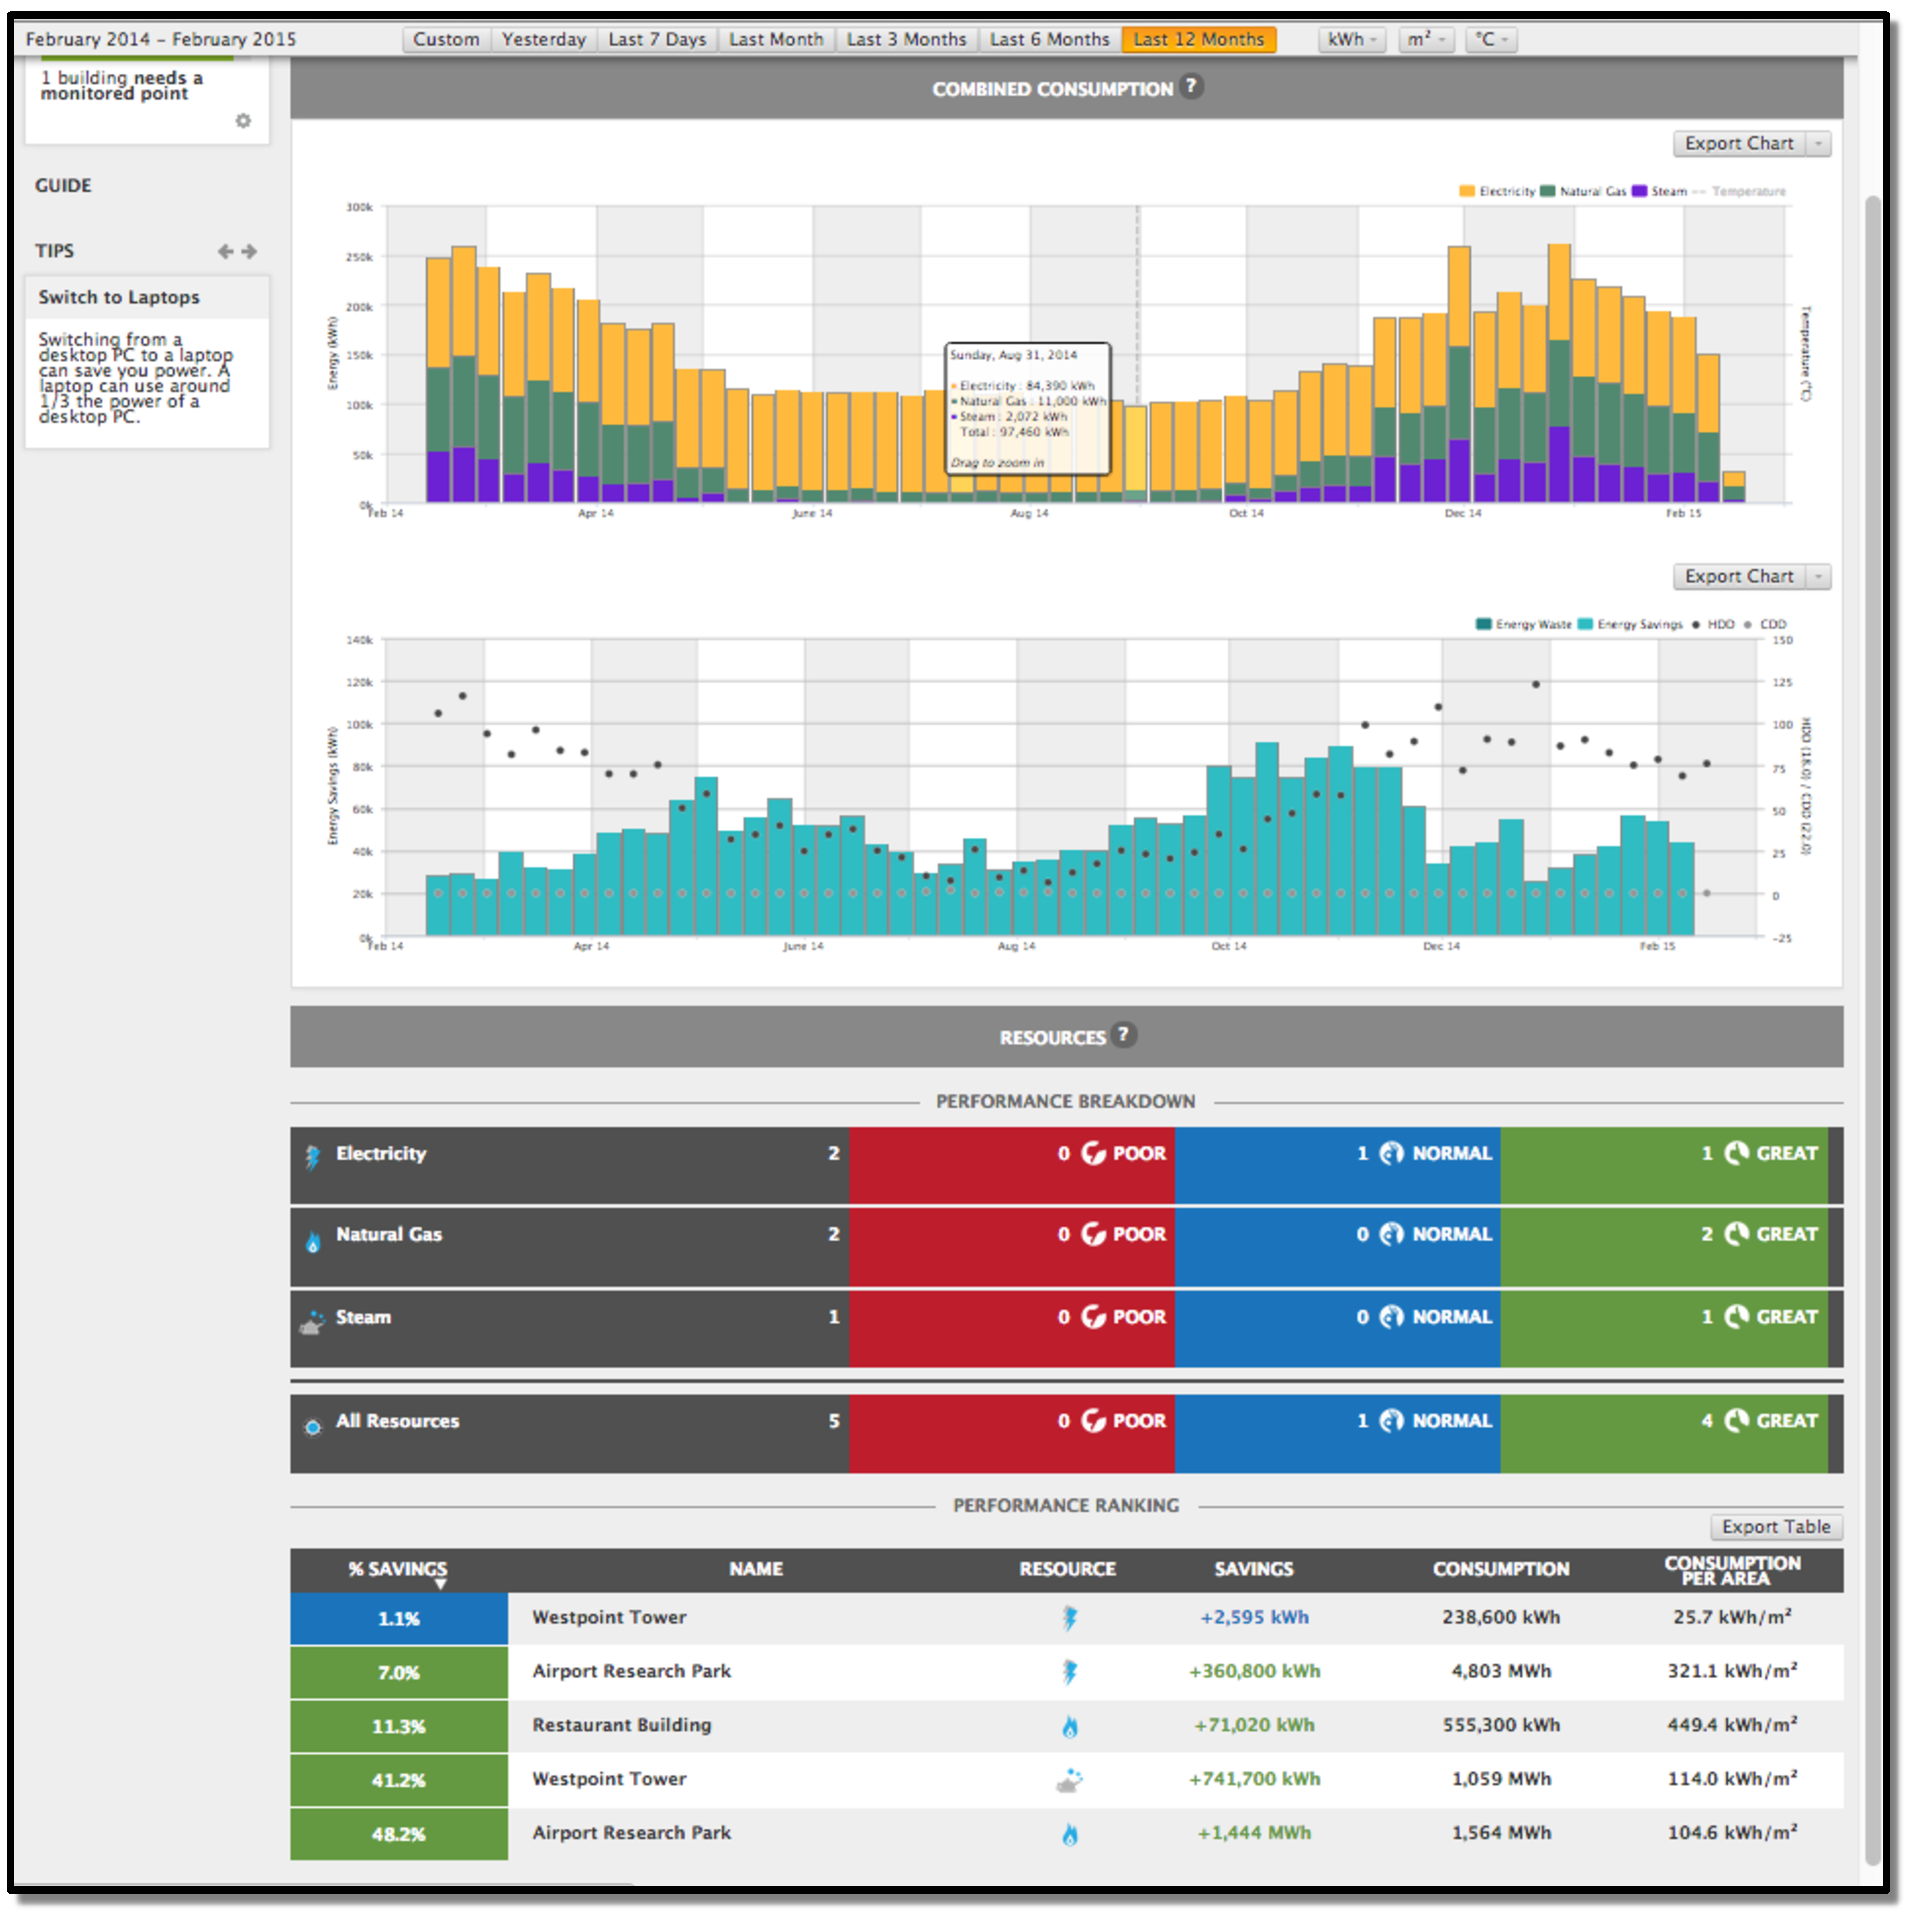
\includegraphics[width=\textwidth]{figures/em-top.pdf}
	\caption
	[
	    The previous version of Energy Manager, our collaborators' energy analysis tool.
	]
	{
	    The previous version of Energy Manager, our collaborators' energy analysis tool: a dashboard for a portfolio of buildings.
	}
	\centering
	\label{emu:fig:energy-manager-top}
\end{figure} 

%-|-|-|-|-|-|-|-|-|-|-|-|-|-|-|-|-|-|-|-|-|-|-|-|-|-|-|-|-|-|-|-|-|-|-|-|-

%-|-|-|-|-|-|-|-|-|-|-|-|-|-|-|-|-|-|-|-|-|-|-|-|-|-|-|-|-|-|-|-|-|-|-|-|-

\begin{figure}
	\centering
	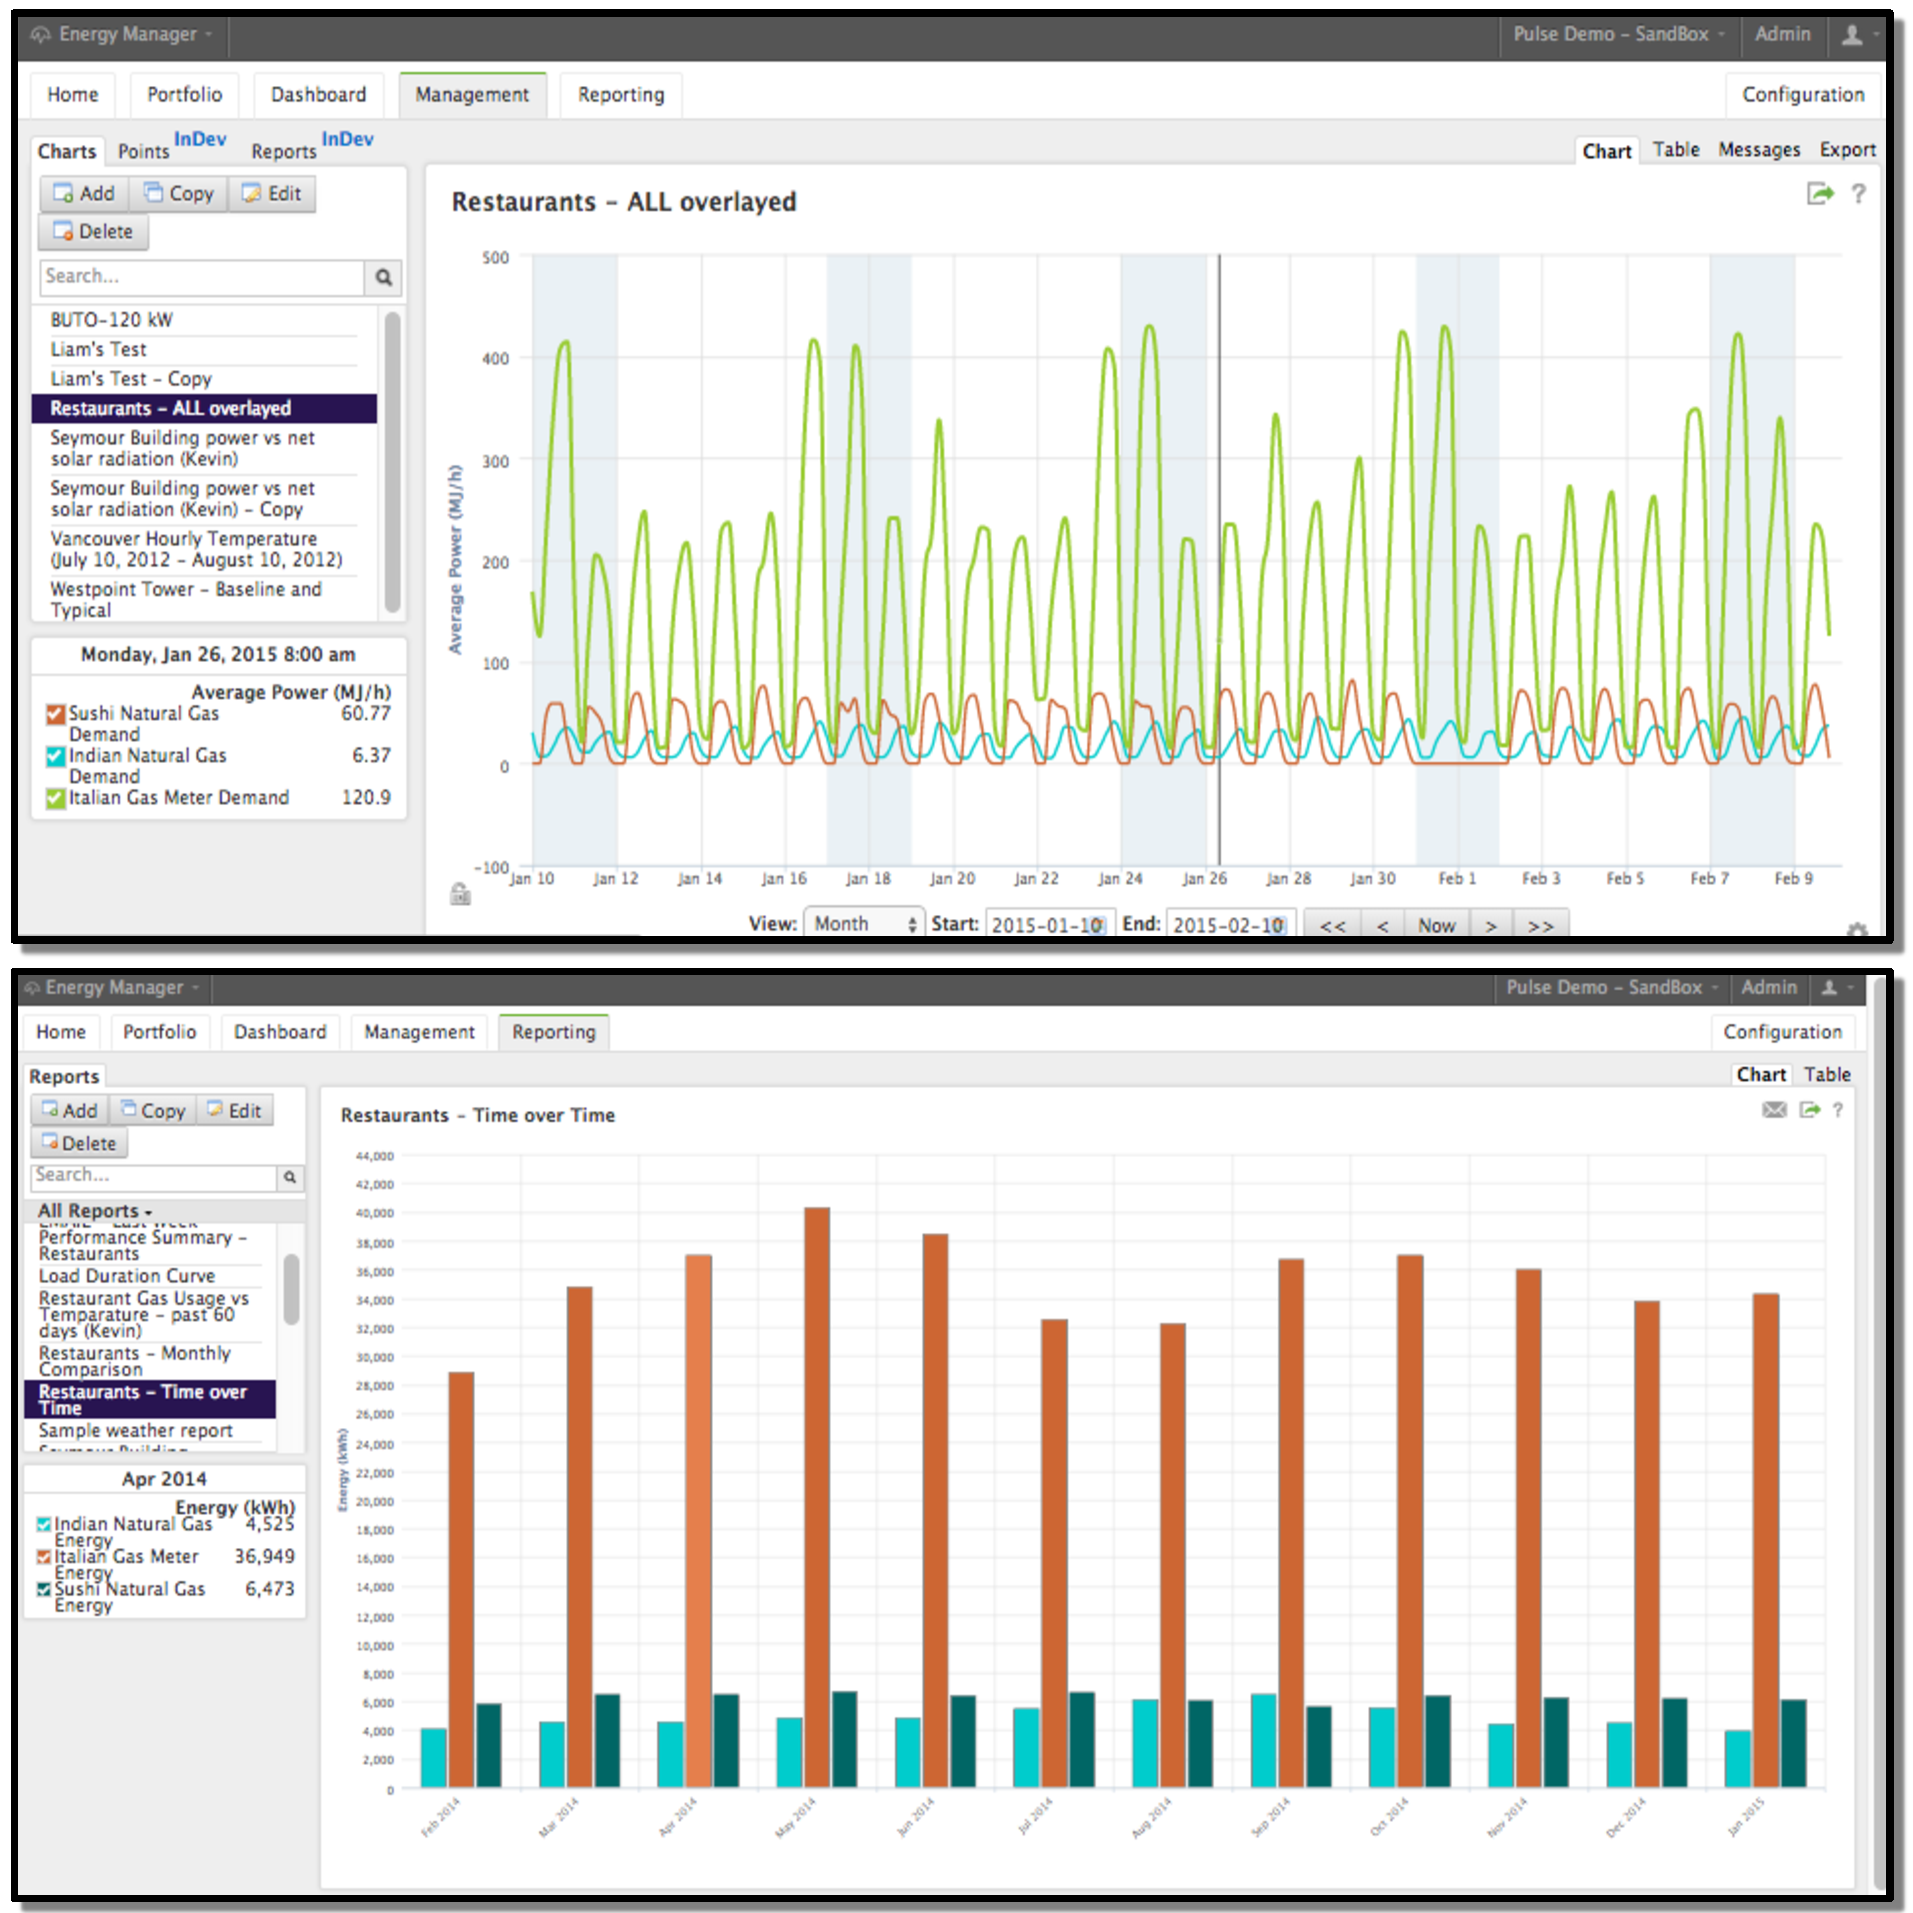
\includegraphics[width=\textwidth]{figures/em-bottom.pdf}
	\caption
	[
	    The previous version of Energy Manager, our collaborators' energy analysis tool (continued).
	]
	{
	    The previous version of Energy Manager, our collaborators' energy analysis tool (continued). A superimposed line graph of \textsl{energy demand} (top) and a grouped bar chart of \textsl{energy consumption} (bottom) for a group of three restaurant buildings within this portfolio.
	}
	\centering
	\label{emu:fig:energy-manager-bottom}
\end{figure} 

%-|-|-|-|-|-|-|-|-|-|-|-|-|-|-|-|-|-|-|-|-|-|-|-|-|-|-|-|-|-|-|-|-|-|-|-|-

Line graphs\index{visual encoding!line graph} and bar charts\index{visual encoding!bar chart} such as those in \autoref{emu:fig:energy-manager-bottom} (top) and \autoref{emu:fig:energy-manager-bottom} (bottom) are indexed on the other pages, similar to how a Microsoft Excel\index{Excel (Microsoft)} workbook has sheets, which can in turn contain multiple charts. 
Unlike Excel\index{Excel (Microsoft)}, Energy Manager's\index{Energy Manager} charts provide some interactivity: an energy analyst can zoom, pan, and reveal values upon mouseover. 
However, none of the charts are directly linked to one another or to the dashboard, so the energy analyst must {\tt navigate}\index{{\tt navigate}} between them manually.

\bstart{Task support} Energy Manager\index{Energy Manager} only partially supports the Overview ({\bf T1}) task\index{task}: with the portfolio dashboard (\autoref{emu:fig:energy-manager-top}), the energy analyst can observe the aggregate {\it consumption} for a portfolio over time, or alternatively she can observe single aggregate values for individual buildings in the sortable table, but she will not be able to directly {\tt compare}\index{{\tt compare}} how individual buildings vary over time.
As a result, the energy analysts that we interviewed essentially ignored this dashboard, and none of them had found the sortable table to be useful. 

The Drill Down ({\bf T2}) task\index{task} is supported but the current approach used by Energy Manager\index{Energy Manager} does not scale.
The examples in \autoref{emu:fig:energy-manager-bottom} (top) and \autoref{emu:fig:energy-manager-bottom} (bottom) respectively display {\it energy demand} and {\it consumption} performance for three restaurants.
Since superimposed line graphs\index{visual encoding!line graph!superimposed line graph} and grouped bar charts\index{visual encoding!bar chart!grouped bar chart} are limited by the number of discriminable colours, these charts are inappropriate for the energy analyst who needs to consider more than a handful of buildings.

The Roll Up ({\bf T3}) task\index{task} is not explicitly supported. Though it is possible to estimate the proportion of a building's energy performance relative to its group with bars and lines, this process is error-prone.

\bstart{Task sequences not supported}\index{task!task sequence} Because the line graphs\index{visual encoding!line graph}, bar charts\index{visual encoding!bar chart}, and tables in Energy Manager\index{Energy Manager} are not coordinated or linked in any way, it is difficult and tedious to alternate from Overview ({\bf T1}) to Drill Down ({\bf T2}) and Roll Up ({\bf T3}) tasks\index{task}. 
As in Excel\index{Excel (Microsoft)}, the energy analyst will have to {\tt locate}\index{{\tt locate}} an existing chart or specify a new chart using a wizard dialog; if the bar or line graph\index{visual encoding!line graph} for a set of buildings does not already exist when the energy analyst needs it, she has to create it. 
By the time she has created it, she may have forgotten her objective\footnote{Task sequences such as these are likely to be poorly supported in most interactive system that involves wizard dialogs.}.

\bstart{Limited filtering and aggregation} The bar charts\index{visual encoding!bar chart} and line graphs\index{visual encoding!line graph} in Energy Manager\index{Energy Manager} allow an energy analyst to hide or show individual buildings.
However, the energy analyst cannot {\tt filter} \index{{\tt filter}} buildings with shared attributes, such as {\tt filtering}\index{{\tt filter}} a portfolio of buildings to only show restaurants.
Similarly, it is impossible to aggregate buildings together when they share attributes: for instance, the energy analyst cannot {\tt compare}\index{{\tt compare}} the aggregate energy performance of restaurants in one city to those in another city.

\bstart{No faceting} Aside from the seldom-used portfolio dashboard shown in \autoref{emu:fig:energy-manager-top}, there is no faceting\index{view coordination!faceting (small multiples)} or juxtaposition\index{view coordination!view juxtaposition} of charts in Energy Manager\index{Energy Manager}: the energy analysts' workarounds included opening multiple browser windows, adjusting the line or bar charts\index{visual encoding!bar chart} to display the same scale and ranges, and tiling these windows manually across their monitor. 
Similarly, one energy analyst that we spoke to printed and taped charts together to accomplish the same result.

\bstart{Summary} Due to these limitations, energy analysts can only observe narrow slices of their portfolio data, or they are presented with aggregate data that is too coarse to be useful.
In addition, they did not trust Energy Manager's\index{Energy Manager} derived predicted values based on statistical models, and would have preferred to {\tt compare}\index{{\tt compare}} observed energy performance to historical values.
In other words, the derived and aggregated values currently shown may hide information such as extreme values and unusual distributions.
As a result of this loss of detail, energy analysts routinely export tabular data from Energy Manager\index{Energy Manager} and {\tt import}\index{{\tt import}} it into Excel\index{Excel (Microsoft)}, with which they would conduct a time-consuming custom analysis.
Finally, many of the energy analysts to whom we spoke remarked that energy analysis software tools\footnote{\eg Energent EMIS: \url{http://energent.com/emis/}, Northwrite Energy Expert: \url{http://northwrite.com/energyexpert.asp}, Schneider Electric PowerLogic Ion EEM: \url{http://goo.gl/Nh7mJv}} built by our collaborators' competitors have limitations similar to those of Energy Manager\index{Energy Manager}.
Altogether, these problems may help to explain why the number of energy analysts who actively use Energy Manager\index{Energy Manager} is substantially less than the number of client accounts.

%-------------------------------------------------------------------------
%-------------------------------------------------------------------------

\section{Related Work}
\label{emu:related-work}

%-------------------------------------------------------------------------
%-------------------------------------------------------------------------

We now review relevant previous work, beginning with work in the energy domain\index{energy management}. 
We also discuss the visualization of time-oriented data\index{time-oriented data} in other domains, as well as evaluation\index{evaluation} studies that assess the effectiveness of visualization design choices for similar data\index{data abstraction} and task abstractions\index{task!task abstraction}.

\bstart{Visualization in the energy domain} Technology that allows for the continuous measurement of a building's energy demand is becoming increasingly available, and several techniques to monitor and present this data have recently been proposed, especially for residential buildings~\cite{Ellegard2011,Erickson2013,Goodwin2013,Rodgers2011}.
\citet{Erickson2013} developed a web-based residential energy dashboard for homeowners, allowing them to {\tt compare}\index{{\tt compare}} against their neighbours with familiar\index{familiarity} bar charts\index{visual encoding!bar chart} and line graphs\index{visual encoding!line graph}.
However, such a dashboard would be unsuitable for the work of an energy analyst who oversees a portfolio of many buildings.

Though bar chart\index{visual encoding!bar chart} and line graph\index{visual encoding!line graph} depictions of energy data are most common, other visual encodings\index{visual encoding} have also been employed, from abstract and artistic ambient visual encodings~\cite{Rodgers2011}\index{visual encoding} to a compelling calendar-based visual encoding~\cite{VanWijk1999}\index{visual encoding!matrix!calendar (matrix)}, in which calendar dates with similar energy behaviour are visually associated using a common colour.
We also explore visual encodings\index{visual encoding} beyond bar charts\index{visual encoding!bar chart} and line graphs\index{visual encoding!line graph}, and in \autoref{emu:design-matrix}, we consider how to {\tt encode}\index{{\tt encode}} data from multiple buildings using calendars\index{visual encoding!matrix!calendar (matrix)}.
Another approach to {\tt summarizing}\index{{\tt summarize}} the energy behaviour of multiple buildings is to use map-based visual encoding\index{visual encoding!map}, though we discuss the limitations of this approach in \autoref{emu:design-map}. 

More closely related to our work is that of \citet{Goodwin2013}, who visualized modelled residential energy use across thousands of households at the scale of individual household appliances, resulting in four prototype data sketches\index{data sketch}. 
The domain activities they address overlap partially with those performed by the energy analysts we spoke to, such as the need to find anomalous energy performance across many buildings; another activity they address, in which energy modelers perform energy load-shifting simulations to estimate potential savings, is not an activity performed by our energy analysts. 
Their designs incorporated several visual encodings\index{visual encoding} not typically seen in the energy management\index{energy management} domain: horizon graphs~\cite{Heer2009}\index{visual encoding!horizon graph}, boxplots~\cite{Wickham2011}\index{visual encoding!boxplots}, and matrix-based encodings\index{visual encoding!matrix}.
However, the focus and main contribution of their paper was on creative methods for visualization requirements analysis, rather than on a thorough analysis of their visual encoding\index{visual encoding} and interaction\index{interaction} design choices.
In our work, we reexamine some of these visual encodings\index{visual encoding}, among others, and evaluate\index{evaluation} their effectiveness in the context of our data\index{data abstraction} and task abstractions\index{task!task abstraction}. 

\bstart{Visualizing multiple time series} Many techniques for visualizing time-oriented data\index{time-oriented data} have been proposed, and a survey of these techniques by \citet{Aigner2011} has provided us with a structured way to think about this design space.
In their terminology, our designs incorporate {\it linear} and {\it cyclic} encodings of time, depicting {\it abstract multivariate interval} data.

Another axis on which we can analyze existing techniques is the number of time series\index{time-oriented data} being considered.
At the low end of this continuum, superimposed line graphs\index{visual encoding!line graph!superimposed line graph} or grouped bar charts\index{visual encoding!bar chart!grouped bar chart} are appropriate for a small number of time series\index{time-oriented data}. 
In the middle of this continuum, faceting\index{view coordination!faceting (small multiples)} techniques such as faceted\index{view coordination!faceting (small multiples)} line graphs\index{visual encoding!line graph}, horizon graphs~\cite{Heer2009}\index{visual encoding!horizon graph} and matrix-based encodings~\cite{Hao2007,Shimabukuro2004}\index{visual encoding!matrix} are appropriate.
At the high end of this continuum, dense multi-form faceting\index{view coordination!faceting (small multiples)} techniques and those that aggregate time series\index{time-oriented data} together are appropriate when dealing with thousands of time series\index{time-oriented data}, such as in LiveRAC~\cite{McLachlan2008} or Line Graph Explorer~\cite{Lam2007}\footnote{LiveRAC and LGE were both developed by members of our group.}. 
Since we are addressing portfolios of dozens to hundreds of buildings, we position our designs toward the middle of this continuum, and we evaluate\index{evaluation} faceting\index{view coordination!faceting (small multiples)} and matrix-based\index{visual encoding!matrix} approaches in the following section.

\bstart{Evaluation of visualization techniques for time-oriented data}\index{time-oriented data} We also situate our work with regards to experimental studies~\cite{Albers2014,Correll2012,Fuchs2013,Javed2010} that have examined the viability of alternative visual encodings\index{visual encoding} for abstract tasks\index{task!task abstraction} similar to those that we classified: {\tt identifying}\index{{\tt identify}} and {\tt comparing}\index{{\tt compare}} averages, trends, extreme values, and outliers.
Some studies address the viability of encodings for a single time series~\cite{Albers2014,Correll2012}\index{time-oriented data}, while others consider multiple concurrent time series\index{time-oriented data}; one study considered up to sixteen time series~\cite{Javed2010}\index{time-oriented data}, while another considered forty-eight~\cite{Fuchs2013}.
We too assessed the viability of different visual encodings\index{visual encoding} for multiple concurrent time series\index{time-oriented data}; however, our approach involves a qualitative evaluation\index{evaluation} (see \autoref{emu:methodology}), as opposed to a controlled experiment.

Moreover, while these studies considered continuous time series\index{time-oriented data} data, we must consider alternative scalable encodings, since in our case domain conventions\index{domain convention} dictate that continuous line graph\index{visual encoding!line graph} encodings would be misleading for the display of derived and aggregated time series\index{time-oriented data} values, as discussed in \autoref{emu:data-abstractions}.

%-------------------------------------------------------------------------
%-------------------------------------------------------------------------

\section{Prototyping Environments}
\label{emu:sandbox}

%-------------------------------------------------------------------------
%-------------------------------------------------------------------------

\bstart{Shiny sandbox}
We developed an interactive browser-based visualization design sandbox\footnote{\url{http://mattbrehmer.shinyapps.io/PortfolioSandbox}} to produce {\it data sketches}~\cite{Lloyd2011}\index{data sketch}, shown in \autoref{emu:fig:sandbox}. 
The sandbox allowed us to rapidly prototype different visual encoding\index{visual encoding} designs and conduct chauffeured demos\index{chauffeured demos} with energy analysts, a process that we described in \autoref{emu:methodology}. 
All of the designs discussed in \autoref{emu:design:visenc} were produced within this environment, which was developed\footnote{\url{http://github.com/mattbrehmer/PortfolioSandbox}} using the Shiny web application framework\footnote{Shiny is a framework for integrating statistical analysis and visualization techniques within an interactive web application; Shiny web applications are implemented using the R statistical programming language. More information is available here: \url{http://shiny.rstudio.com/}}.

%-|-|-|-|-|-|-|-|-|-|-|-|-|-|-|-|-|-|-|-|-|-|-|-|-|-|-|-|-|-|-|-|-|-|-|-|-

\begin{figure}
	\centering
	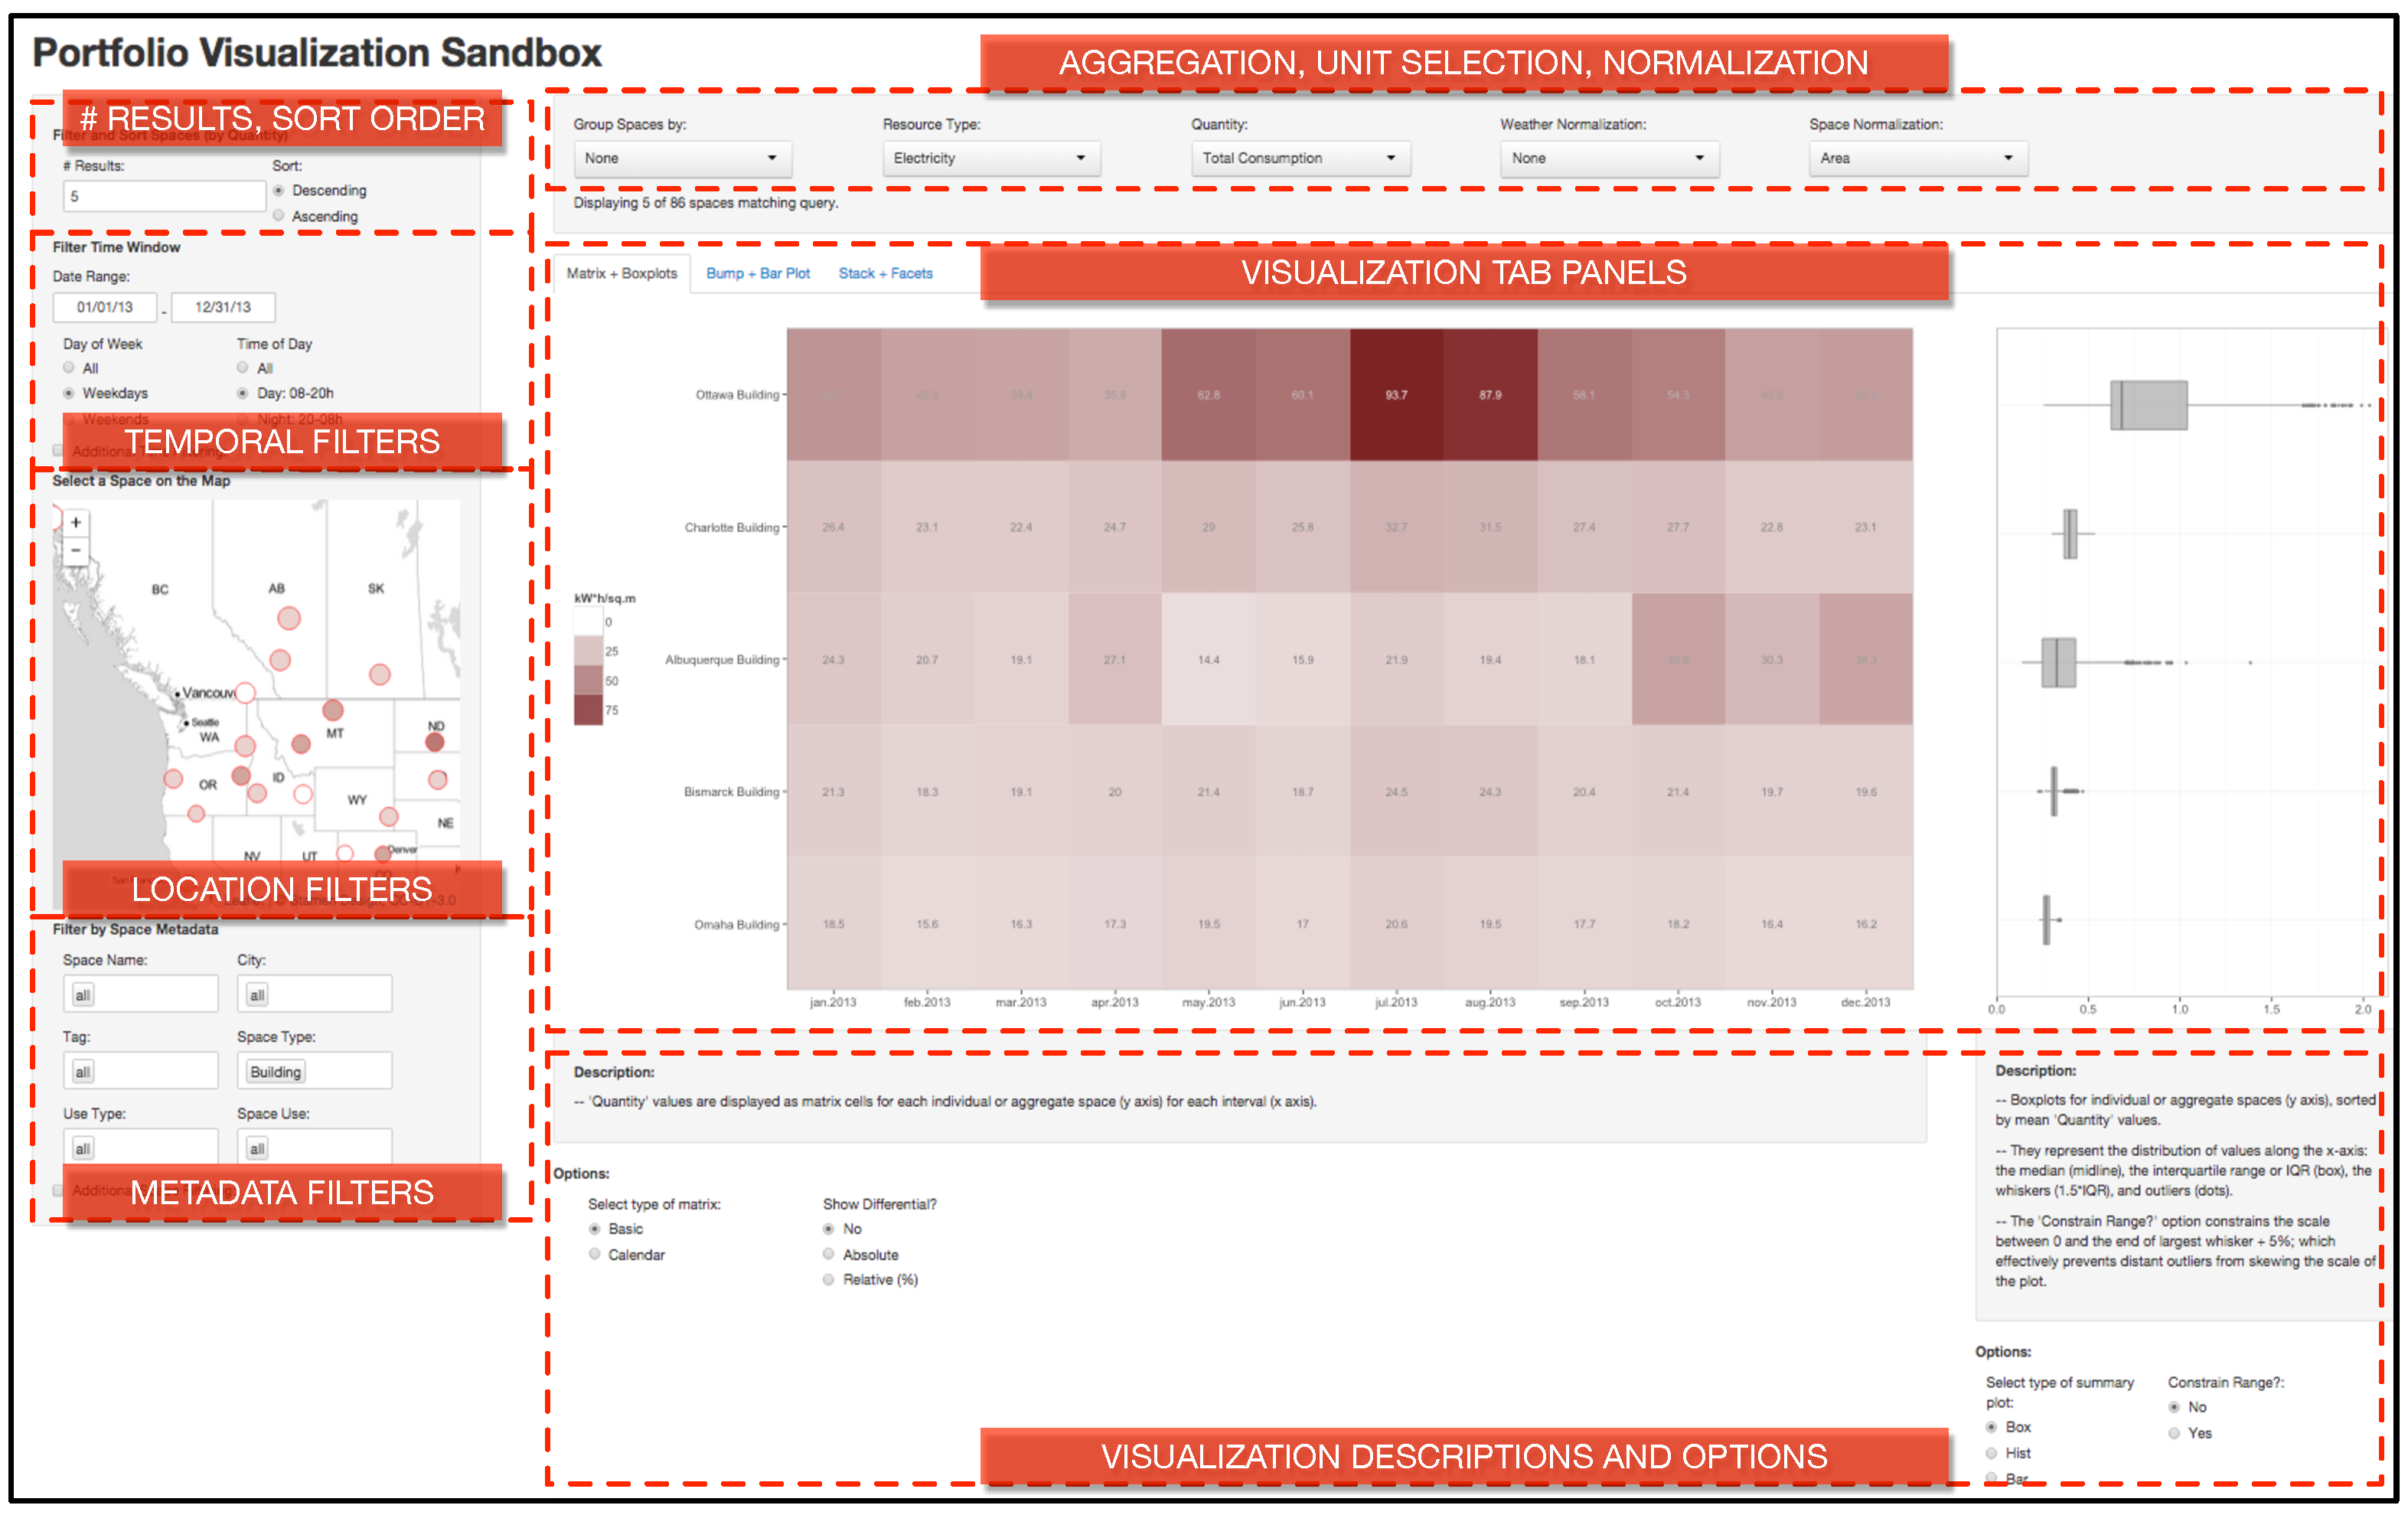
\includegraphics[width=\textwidth]{figures/sandbox.pdf}
	\caption
	[
	    A sandbox design environment for visualizing energy data from a portfolio of buildings.
	]
	{
	    A sandbox design environment for visualizing energy data from a portfolio of buildings. A matrix of aggregate \textsl{energy intensity} values with auxiliary boxplots is shown for 5 (of 86) buildings, those with the highest \textsl{intensity}.
	   % Client portfolio data has been anonymized by changing building names and location; all other data is real.
	}
	\centering
	\label{emu:fig:sandbox}
\end{figure} 

%-|-|-|-|-|-|-|-|-|-|-|-|-|-|-|-|-|-|-|-|-|-|-|-|-|-|-|-|-|-|-|-|-|-|-|-|-

\begin{sloppypar}
This sandbox has interactive controls for sorting ({\tt arranging}\index{{\tt arrange}}), {\tt filtering}\index{{\tt filter}}, and {\tt aggregating} buildings, controls for {\tt selecting}\index{{\tt select}} units of interest such as {\it demand} or {\it consumption}, as well as controls for area and weather normalization; recall that there were no such controls in the Energy Manager\index{Energy Manager} interface.
Whenever these controls are adjusted, we sort the filtered set of buildings according to the currently selected\index{{\tt select}} energy unit of interest and time span.
The sandbox operator can {\tt select}\index{{\tt select}} the number of results to show and sort ({\tt arrange})\index{{\tt arrange}} them. 
For instance, \autoref{emu:fig:sandbox} shows a view described in \autoref{emu:design-matrix}, and in it we show 5 buildings from a geographically anonymized portfolio of 86 buildings, those with the highest {\it energy intensity} in 2013. 
\end{sloppypar}

\bstart{D3 interactive prototypes}
Since our Shiny-based sandbox implementation did not allow us to directly experiment with interactions\index{interaction} involving coordinated {\tt selection}\index{{\tt select}} across juxtaposed views\index{view coordination!view juxtaposition}, we developed several interactive prototypes using D3~\cite{Bostock2011} that specifically address this coordination;  these prototypes are discussed in \autoref{emu:design:workflows} and one of them\footnote{\url{http://bl.ocks.org/mattbrehmer/287e44c9a12151967874}} is shown in \autoref{emu:fig:interactive-boxplots}.

%-------------------------------------------------------------------------
%-------------------------------------------------------------------------

\section{Visual Encoding Matches and Mismatches}
\label{emu:design:visenc}

%-------------------------------------------------------------------------
%-------------------------------------------------------------------------

Meyer~\etal's nested blocks and guidelines model~\cite{Meyer2015}, which extends Munzner's nested model~\cite{Munzner2009,Munzner2014}\index{nested model (Munzner)}, describes a need for guidelines that relate the domain, abstraction\index{task!task abstraction}\index{data abstraction}, idiom (visual encoding and interaction design choices), and algorithm levels of visualization design.
In \autoref{emu:abstractions}, we described the relationship between domain activities and the data\index{data abstraction} and task abstractions\index{task!task abstraction}.
In this section, we consider the space of visual encoding\index{visual encoding} design choices and present guidelines for matching design choices to abstractions\index{task!task abstraction}\index{data abstraction}. 
Since the space of possible visual encoding\index{visual encoding} design choices for time-oriented data\index{time-oriented data} is large~\cite{Aigner2011}, we undertook a typical design study\index{design studies} approach~\cite{Sedlmair2012}: considering several design choices, implementing a subset of them, and selecting only the few good matches.

We identified five {\it matches} \{\match\} between visual encoding\index{visual encoding} design choices and the combination of data\index{data abstraction} and task abstractions\index{task!task abstraction}, based on evidence resulting from our process described in \autoref{emu:methodology}. 
We also identified four {\it mismatches} \{\mismatch\} and two {\it potential matches} \{\posmatch\}. 
These matches and mismatches, indicated in \autoref{emu:tab:matches-mismatches}, serve as guidelines that are transferable beyond the energy management\index{energy management} domain, especially when we consider the similarity between our abstract tasks\index{task!task abstraction} to those addressed in domain-agnostic evaluation\index{evaluation} studies~\cite{Albers2014,Javed2010}.
Furthermore, these matches and mismatches fill a gap with regards to identifying suitable visual encoding\index{visual encoding} design choices for multiple time series\index{time-oriented data} in which values are not continuous, but derived and aggregated values that should {\it not} be {\tt encoded}\index{{\tt encode}} as line graphs\index{visual encoding!line graph}.

%-|-|-|-|-|-|-|-|-|-|-|-|-|-|-|-|-|-|-|-|-|-|-|-|-|-|-|-|-|-|-|-|-|-|-|-|-

\begin{table}\renewcommand{\arraystretch}{1.2}\addtolength{\tabcolsep}{-1pt}
    \begin{center}
    \scriptsize
    \begin{tabular}{l|l|c}

        \rowcolor{blue!15}
    
        {\bf Task} & {\bf Design Choice} & {\bf Match?}
        
        \\
        
        %task
        {\bf T1}: Overview 
        
        %idiom
        & Faceted\index{view coordination!faceting (small multiples)} bar chart\index{visual encoding!bar chart} 
        
        %match?
        & \mismatch
        
        \\
        
        \rowcolor{gray!15}
        
        %task
        %{\bf T1}: Overview 
        
        %idiom
        & Bump plot\index{visual encoding!bump plot}
        
        %match?
        & \mismatch
        
        \\
        
        %task
        %{\bf T1}: Overview 
        
        %idiom
        & Bar + bump plot\index{visual encoding!bar + bump plot} 
        
        %match?
        & \posmatch
        
        \\
        
        \rowcolor{gray!15}

        %task
        %{\bf T1}: Overview 
        
        %idiom
        & (Calendar) matrix\index{visual encoding!matrix!calendar (matrix)} 
        
        %match?
        & \posmatch
        
        \\
        
        %task
        %{\bf T1}: Overview 
        
        %idiom
        &Map\index{visual encoding!map}
        
        %match?
        & \mismatch
        
        \\
        
        \rowcolor{gray!15}
        
        %task
        %{\bf T1}: Overview 
        
        %idiom
        & Juxtaposed\index{view coordination!view juxtaposition} matrix\index{visual encoding!matrix} and boxplots\index{visual encoding!boxplots} 
        
        %match?
        & \match
        
        \\
        
        
        \hline
        
        %task
        
        {\bf T2}: Drill Down 
        
        %idiom
        & Faceted\index{view coordination!faceting (small multiples)} bar chart\index{visual encoding!bar chart} 
        
        %match?
        & \match
        
        \\
        
        \rowcolor{gray!15}
        
        %task
        %{\bf T2}: Drill Down 
        
        %idiom
        & Faceted\index{view coordination!faceting (small multiples)} boxplot\index{visual encoding!boxplots} 
        
        %match?
        & \mismatch
        
        \\
        
        %task
        %{\bf T2}: Drill Down 
        
        %idiom
        & Faceted\index{view coordination!faceting (small multiples)} line graph\index{visual encoding!line graph} 
        
        %match?
        & \match
        
        \\
        
        \rowcolor{gray!15}
        
        \hline
        
        %task
        {\bf T3}: Roll Up 
        
        %idiom
        & Stacked area graph\index{visual encoding!stacked area graph} 
        
        %match?
        & \match
        
        \\
        
        %task
        %{\bf T3}: Roll Up 
        
        %idiom
        & Stacked bar chart\index{visual encoding!bar chart!stacked bar chart} 
        
        %match?
        & \match
        
        \\
        
        \hline  
        
    \end{tabular}
    \caption
    [
        A summary of the \textsl{matches} and \textsl{mismatches} between abstract tasks and visual encoding design choices.
    ]
    {
        A summary of the \textsl{matches} and \textsl{mismatches} between abstract tasks and visual encoding design choices.
    }
    \label{emu:tab:matches-mismatches}
    \end{center}
\end{table}

%-|-|-|-|-|-|-|-|-|-|-|-|-|-|-|-|-|-|-|-|-|-|-|-|-|-|-|-|-|-|-|-|-|-|-|-|-

%-------------------------------------------------------------------------

\subsection{Faceted Views for Overview and Drill Down}
\label{emu:design-faceting}

%-------------------------------------------------------------------------'

We initially thought that faceted ``small multiple'' views\index{view coordination!faceting (small multiples)} would be a good match for {\it both} the Overview ({\bf T1}) and Drill Down ({\bf T2}) tasks\index{task}, in that they provide a scalable alternative to grouped bar charts\index{visual encoding!bar chart} and superimposed line graphs\index{visual encoding!line graph!superimposed line graph}.

\bstart{Faceted bar charts} {\it a mismatch} \{\mismatch\} {\it for the} Overview ({\bf T1}) {\it task, yet a match} \{\match\} {\it for the} Drill Down ({\bf T2}) {\it task}.
Faceted\index{view coordination!faceting (small multiples)} bar charts\index{visual encoding!bar chart} were among the first designs that we considered, especially after one energy analyst provided us with his own mockup of such a design.
However, if an energy analyst has dozens or hundreds of buildings in their portfolio, faceting\index{view coordination!faceting (small multiples)} is unlikely to scale~\cite{Javed2010}. 
We determined that it was a poor match for the Overview ({\bf T1}) task\index{task}, though a match for the Drill Down ({\bf T2}) task\index{task}, provided that the energy analyst has already {\tt filtered}\index{{\tt filter}} down to a smaller group of buildings, such as {\tt filtering}\index{{\tt filter}} a university portfolio to show only the {\it ``laboratory''} buildings.
In addition, one of the energy analysts lamented that bar charts\index{visual encoding!bar chart} only show coarse aggregate values, typically an average or a sum, and as a result of this loss of detail, they do not show other aggregate values of interest, such as ranges or extreme values within each corresponding time interval.

\bstart{Faceted boxplots}\index{visual encoding!boxplots} {\it a mismatch} \{\mismatch\} {\it for the} Drill Down ({\bf T2}) {\it task}\index{task}.
We expected that faceted\index{view coordination!faceting (small multiples)} boxplots\index{visual encoding!boxplots} would allow energy analysts to {\tt compare}\index{{\tt compare}} ranges, distributions, and extreme values for multiple buildings at different points in time, such as in \autoref{emu:fig:sandbox-faceted-boxplot}.
However, despite the long history of boxplots~\cite{Wickham2011}\index{visual encoding!boxplots} and support from influential visualization practitioners~\cite{Few2014}, we found that most energy analysts are not familiar\index{familiarity} with boxplots\index{visual encoding!boxplots}, except for a minority who had taken a post-secondary statistics course.
Furthermore, comparisons\index{{\tt compare}} in faceted\index{view coordination!faceting (small multiples)} boxplots\index{visual encoding!boxplots} are more difficult than in faceted\index{view coordination!faceting (small multiples)} bar charts\index{visual encoding!bar chart}, where positions are aligned to each facet's baseline; with faceted\index{view coordination!faceting (small multiples)} boxplots\index{visual encoding!boxplots}, the observer must {\tt compare}\index{{\tt compare}} multiple positions and widths across separate facets\index{view coordination!faceting (small multiples)}. 
Our design was therefore a daunting introduction to boxplots\index{visual encoding!boxplots} for those unfamiliar\index{familiarity} with them and a poor match for the Drill Down task\index{task}.

%-|-|-|-|-|-|-|-|-|-|-|-|-|-|-|-|-|-|-|-|-|-|-|-|-|-|-|-|-|-|-|-|-|-|-|-|-

\begin{figure}
	\centering
	\fbox{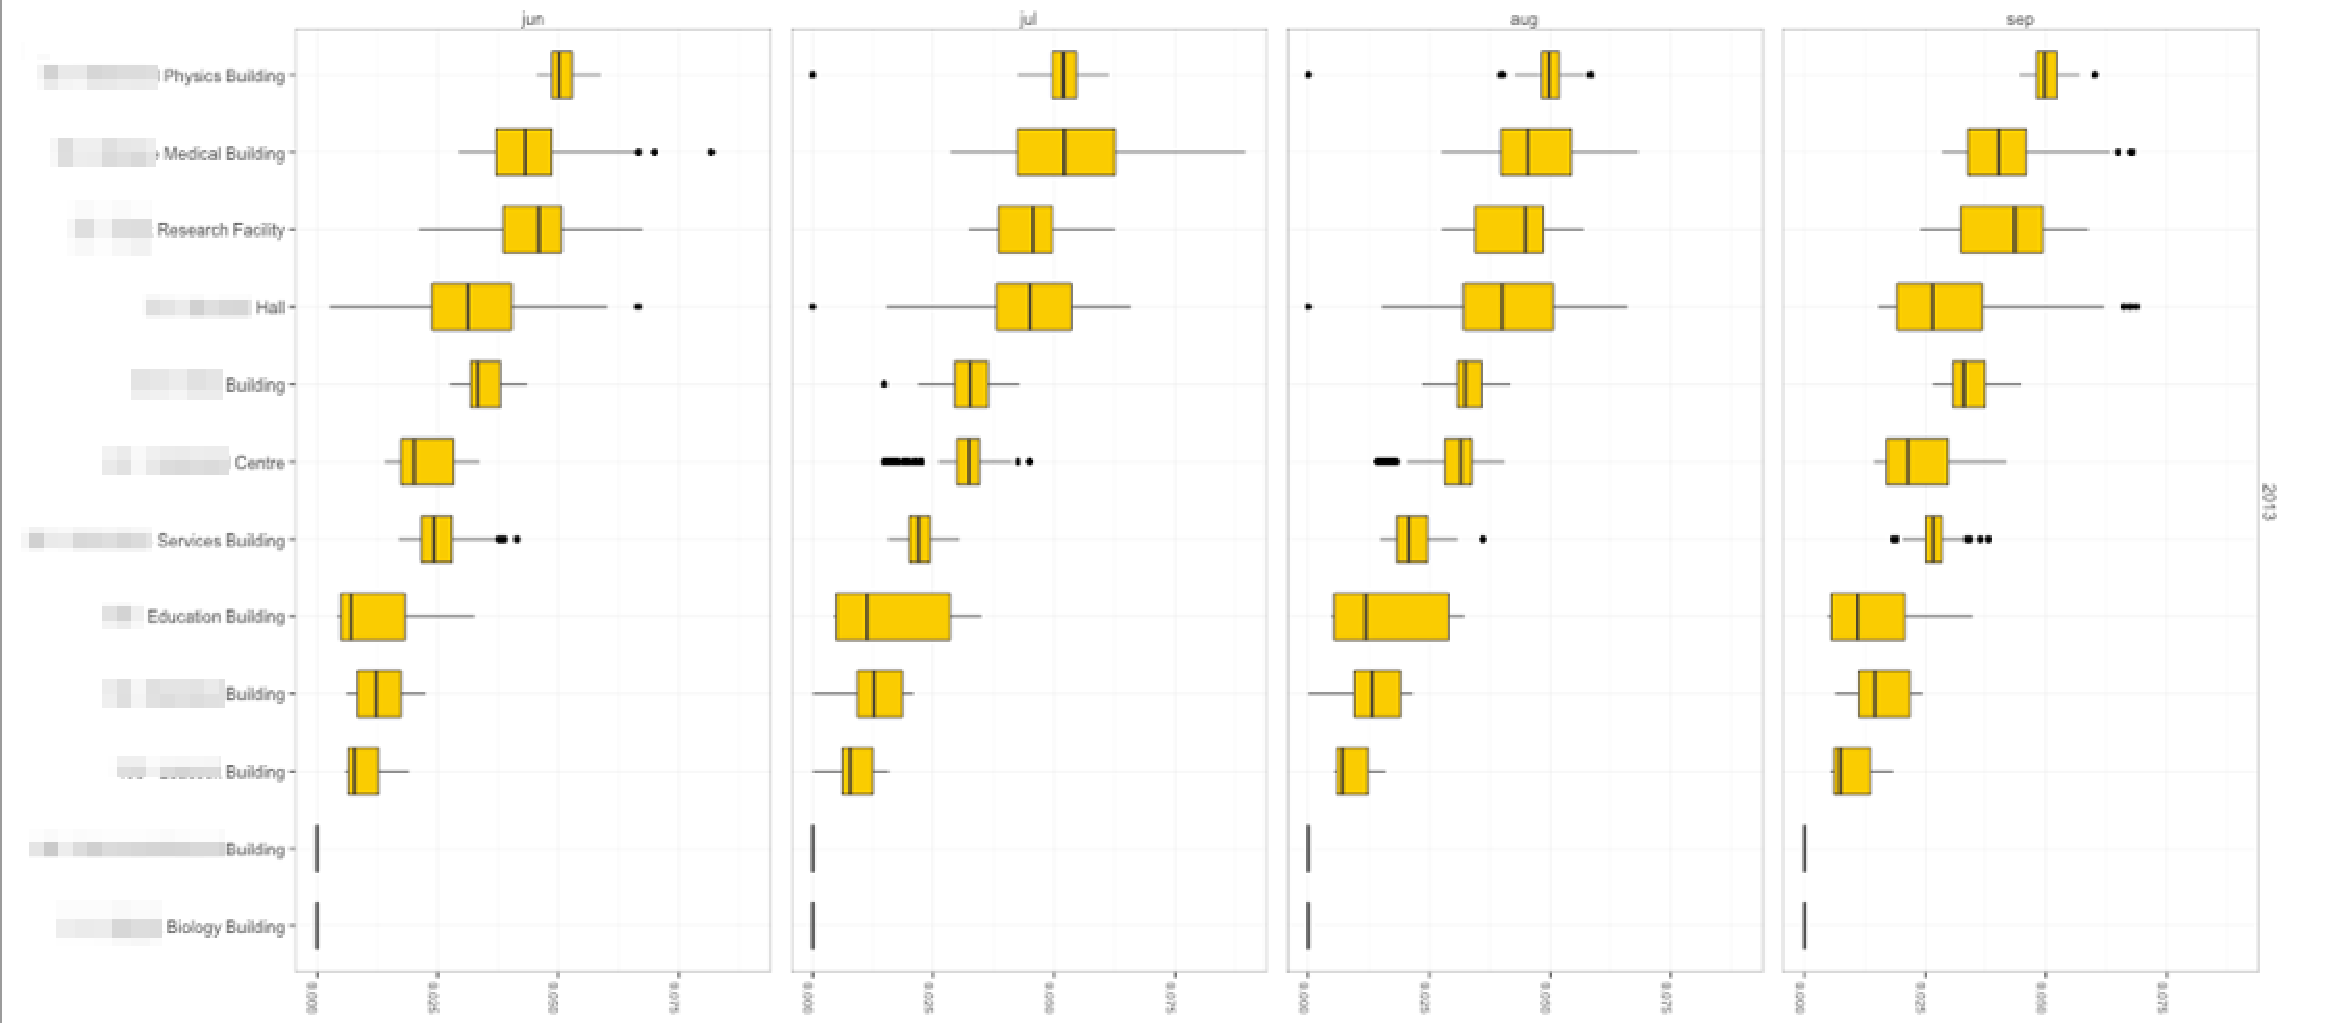
\includegraphics[width=0.975\textwidth]{figures/sandbox-faceted-boxplot.pdf}}
	\caption
	[
	    Faceted boxplots that encode aggregate area-normalized energy \textsl{demand} distributions.
	]
	{
	    Faceted boxplots that {\tt encode} aggregate area-normalized energy \textsl{demand} distributions for twelve buildings across four months, sorted in descending order according to the average \textsl{demand} value for this four month period. Faceted boxplots are a mismatch \{\mismatch\} for the Drill Down task (T2). Building names are blurred to sanitize real client portfolio data.
	}
	\centering
	\label{emu:fig:sandbox-faceted-boxplot}
\end{figure} 

%-|-|-|-|-|-|-|-|-|-|-|-|-|-|-|-|-|-|-|-|-|-|-|-|-|-|-|-|-|-|-|-|-|-|-|-|-

\bstart{Faceted line graphs} {\it a match} \{\match\} {\it for the} Drill Down ({\bf T2}) {\it task}\index{task}.
Faceted\index{view coordination!faceting (small multiples)} line graphs\index{visual encoding!line graph} are a good match when observing non-derived continuous quantitative time series\index{time-oriented data} values such as {\it energy demand}; an example is shown in \autoref{emu:fig:sandbox-stacks} (bottom).
They are a scalable alternative to superimposed line graphs~\cite{Javed2010}\index{visual encoding!line graph} and the line graphs\index{visual encoding!line graph} encoding is already very familiar\index{familiarity} to energy analysts.
As mentioned above in \autoref{emu:abstractions}, line graphs\index{visual encoding!line graph} are {\it not} appropriate for derived and aggregated values such as {\it energy consumption} or {\it intensity}.

%-------------------------------------------------------------------------

\subsection{Rank-Based Overviews}
\label{emu:design-ranking}

%-------------------------------------------------------------------------

As faceting\index{view coordination!faceting (small multiples)} seemed unlikely to be effective for the Overview ({\bf T1}) task\index{task}, we considered non-faceted\index{view coordination!faceting (small multiples)} designs and the encoding of aggregate values.
Recall how the sortable table in Energy Manager's\index{Energy Manager} portfolio dashboard (\autoref{emu:fig:energy-manager-top}, bottom) was never used for the Overview task\index{task}; it contained only coarse aggregate values for each item, providing little detail about temporal variation.
We therefore experimented with encodings for displaying rank as well as rank change over time.

\bstart{Bump plots} {\it a mismatch} \{\mismatch\} {\it for the} Overview ({\bf T1}) {\it task}\index{task}.
Bump plots {\tt encode}\index{{\tt encode}} rank and rank change; they incorporate a familiar\index{familiarity} line encoding across equally-spaced temporal intervals~\cite{Tufte1990}. 
However, as with superimposed line graphs\index{visual encoding!line graph!superimposed line graph}, it becomes difficult to distinguish individual items using colour.
One possible solution is to highlight items that vary in rank, rather than requiring the observer to {\tt locate}\index{{\tt locate}} these items.
Another problem is that bump plots\index{visual encoding!bump plot} only show relative rank and rank change, whereas the absolute values that produce these ranks are not shown. 
Due to this loss of detail, the bump plot\index{visual encoding!bump plot} is also a poor match for the Overview task\index{task}.

\bstart{Bump + bar plots} {\it a potential match} \{\posmatch\} {\it for the} Overview ({\bf T1}) {\it task}\index{task}.
We next considered an encoding that incorporates relative rank, rank change, and absolute value, by adding bars to each series in the bump plot\index{visual encoding!bump plot}, as shown in \autoref{emu:fig:sandbox-barbump}. 
This approach is similar to two recently proposed techniques that {\tt encode}\index{{\tt encode}} both relative rank and absolute value~\cite{Gratzl2013,Hur2013}. 
With this design, we still face the scalability problem associated with colour discriminability.
A combination of interaction\index{interaction} and highlighting rank variation may facilitate this discriminability; in \autoref{emu:fig:sandbox-barbump}, rank variation is encoded using the alpha channel, so the pink series that varies considerably over time is most salient.

%-|-|-|-|-|-|-|-|-|-|-|-|-|-|-|-|-|-|-|-|-|-|-|-|-|-|-|-|-|-|-|-|-|-|-|-|-

\begin{figure}
	\centering
	\fbox{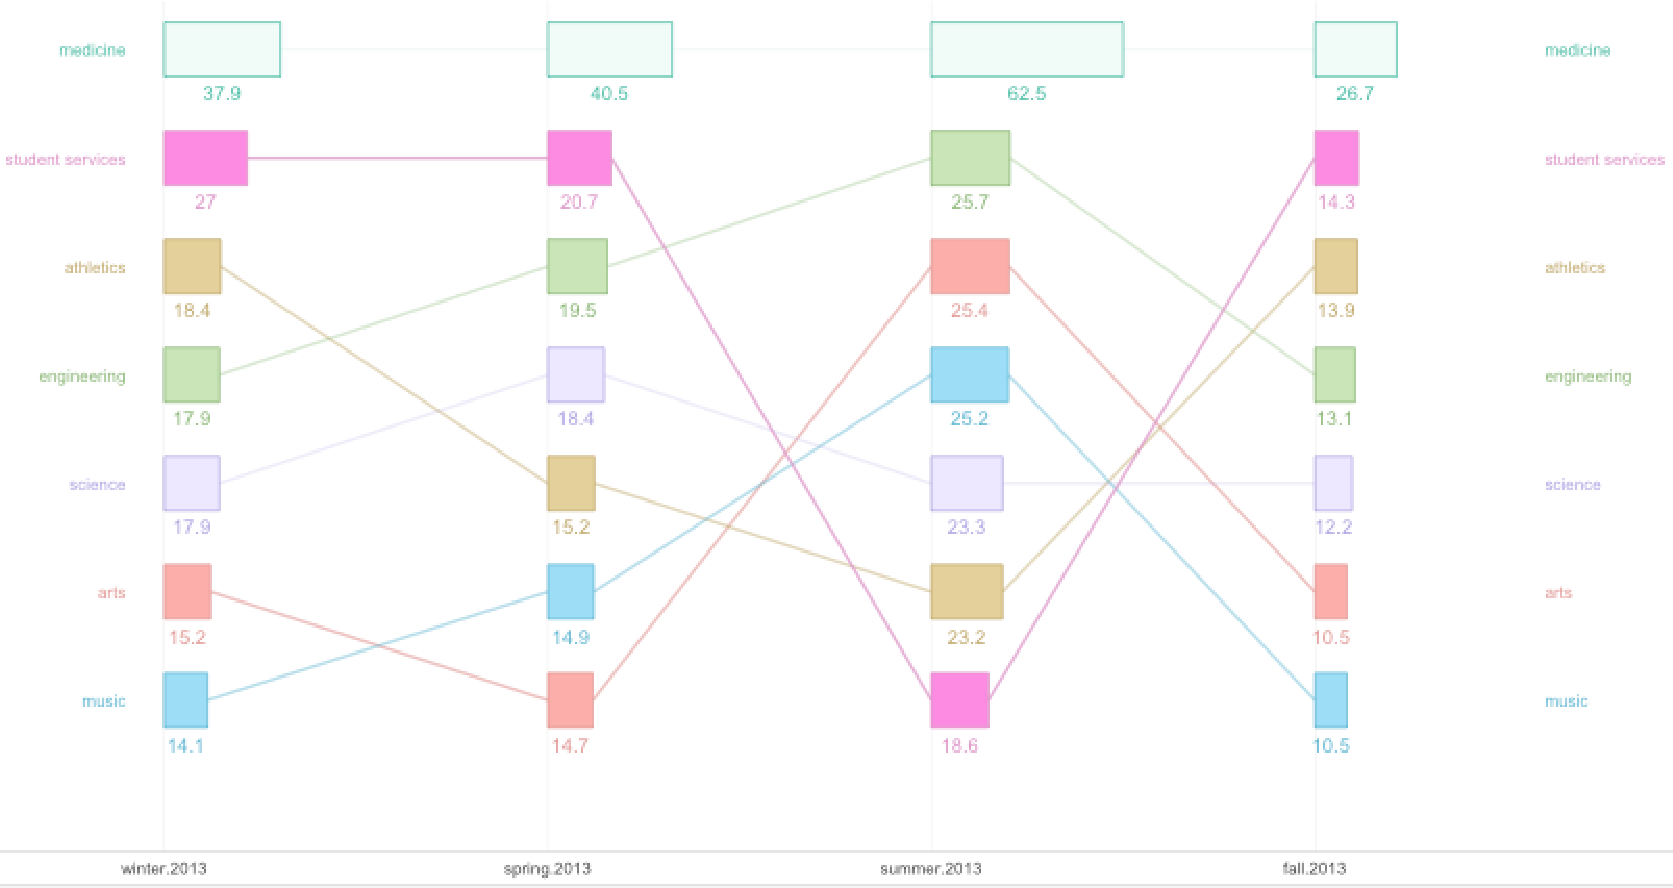
\includegraphics[width=0.975\textwidth]{figures/sandbox-barbump.pdf}}
	\caption
	[
	    A \textsl{bar + bump plot} of \textsl{energy intensity}.
	]
	{
	    A \textsl{bar + bump plot} of \textsl{energy intensity}, encoding rank change for the top seven building groups (buildings aggregated by tag) across four seasons. The alpha channel {\tt encodes} rank variation to highlight inconsistent buildings; in this instance, so the pink series (beginning in the top left) varies considerably over time and is most salient. The \textsl{bar + bump plot} is a potential match  \{\posmatch\} for the Overview task (T1).
	}
	\centering
	\label{emu:fig:sandbox-barbump}
\end{figure}

%-|-|-|-|-|-|-|-|-|-|-|-|-|-|-|-|-|-|-|-|-|-|-|-|-|-|-|-|-|-|-|-|-|-|-|-|-

Energy analysts responded positively to this visual encoding\index{visual encoding}, as it is comprised of familiar\index{familiarity} bar and line encodings. 
However, despite this positive response, we discovered that {\it ranks} as derived values are actually infrequently considered during energy analysis, and that they tend to be more appropriate for annual planning and presentation activities, such as determining how to prioritize energy conservation projects, and less so for recurring analysis and monitoring activities.
Thus, the hunt for a match for the Overview ({\bf T1}) task\index{task} continued.

%-------------------------------------------------------------------------

\subsection{Matrix-Based Overviews}
\label{emu:design-matrix}

%-------------------------------------------------------------------------

\bstart{Time series matrix}\index{visual encoding!matrix} {\it a potential match} \{\posmatch\} {\it for the} Overview ({\bf T1}) {\it task}\index{task}.
Matrix encodings\index{visual encoding!matrix} are scalable and space-efficient~\cite{Goodwin2013,Hao2007}, as can be seen in the center of \autoref{emu:fig:sandbox}.
Matrix encodings\index{visual encoding!matrix} allow us to display observed as well as differential values, allowing an energy analyst to review {\it energy savings} relative to predicted or historical values; a matrix\index{visual encoding!matrix} displaying differential energy data is shown in \autoref{emu:fig:sandbox-calendar}. 
Most of the energy analysts that we interviewed were unfamiliar\index{familiarity} with this form of encoding, except one who had made use of a similar visual encoding\index{visual encoding} in Excel\index{Excel (Microsoft)}. 
As a result, it took more effort to convince our collaborators of the value of these matrix-based encodings\index{visual encoding!matrix} for the Overview task\index{task}.

We also learned that energy analysts found matrices with diverging colour scales easier to interpret than than those with unidirectional colour scales. 
Finally, we found that while red is appropriate for use in diverging colour scales, as it has a negative connotation, it is inappropriate for unidirectional colour scales in this context. 
As a result of this mixed response to matrix-based encodings\index{visual encoding!matrix}, we realized that more work needed to be done.

\bstart{Calendar matrix}\index{visual encoding!matrix!calendar (matrix)} {\it a potential match} \{\posmatch\} {\it for the} Overview ({\bf T1}) {\it task}\index{task}.
We altered our matrix encoding\index{visual encoding!matrix} by partitioning the cells corresponding to months into calendars (\autoref{emu:fig:sandbox-calendar}), a design decision inspired by previous work~\cite{Lammarsch2009,VanWijk1999}. 
Energy analysts responded positively to this encoding, which helped to resolve the unfamiliarity\index{familiarity} of the more generic matrix encoding\index{visual encoding!matrix}. 
However, months and days are not the only time granularities of interest, so this encoding may not be appropriate for all time ranges.

%-|-|-|-|-|-|-|-|-|-|-|-|-|-|-|-|-|-|-|-|-|-|-|-|-|-|-|-|-|-|-|-|-|-|-|-|-

\begin{figure}
	\centering
	\fbox{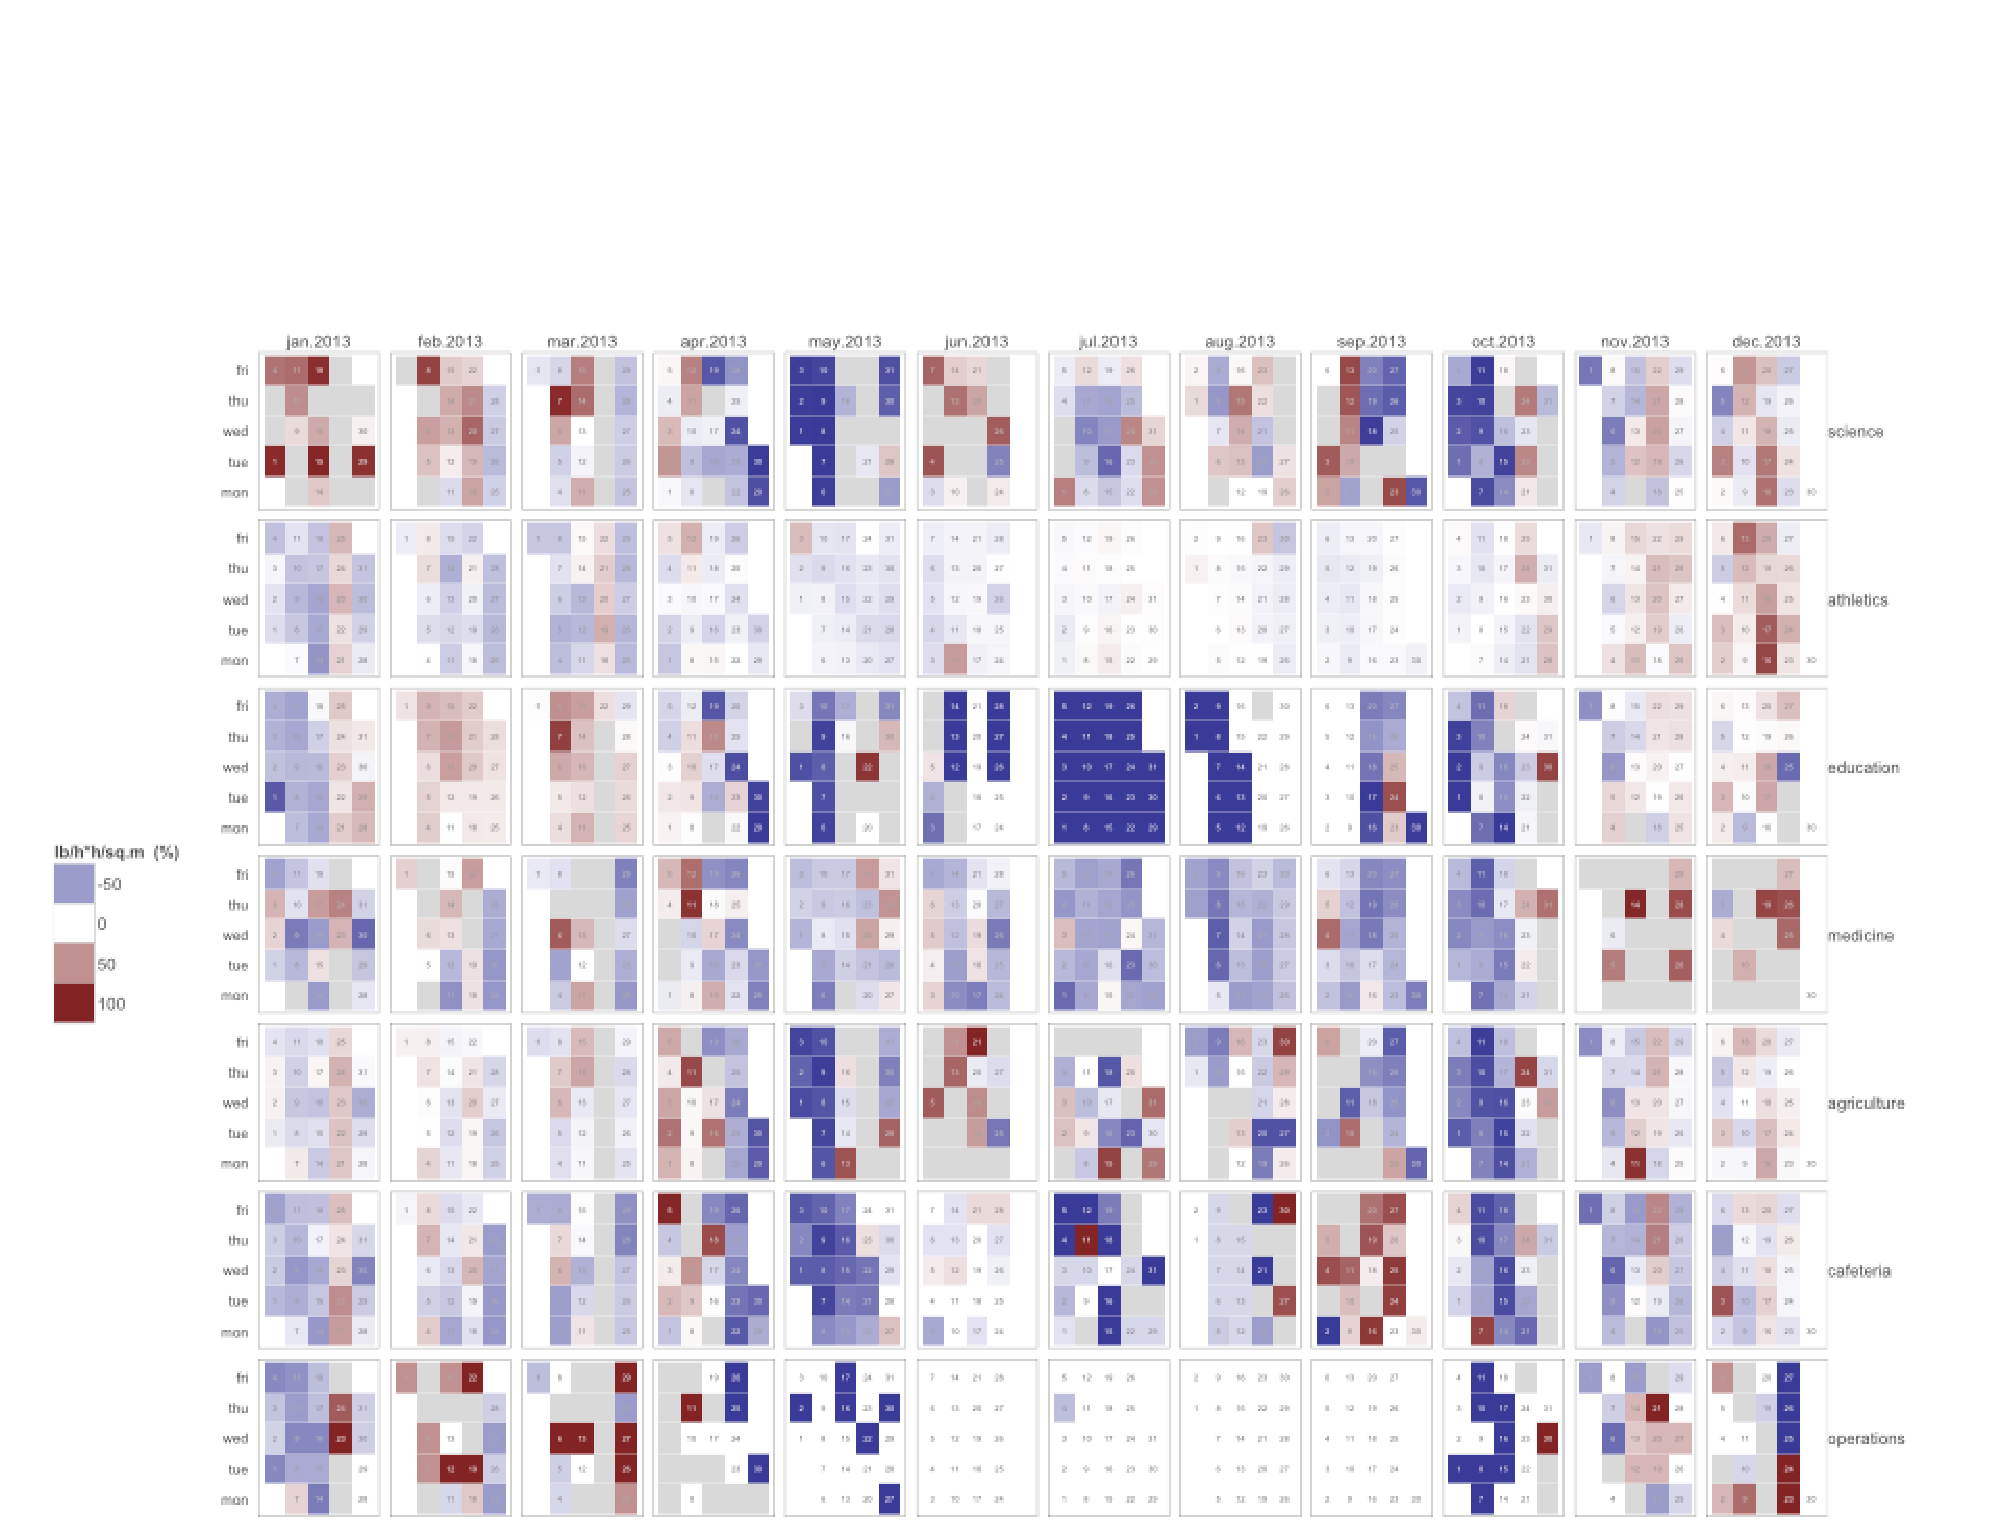
\includegraphics[width=0.975\textwidth]{figures/sandbox-calendar.pdf}}
	\caption
	[
	    A time series calendar matrix of \textsl{energy intensity savings}.
	]
	{
	    A time series calendar matrix of \textsl{energy intensity savings} for seven building groups (buildings aggregated by shared categorical tag), relative to historical values (blue = \textsl{savings}, red = higher than historical \textsl{intensity}). The time series calendar matrix is a potential match \{\posmatch\} for the Overview task (T1).
	}
	\centering
	\label{emu:fig:sandbox-calendar}
\end{figure}

%-|-|-|-|-|-|-|-|-|-|-|-|-|-|-|-|-|-|-|-|-|-|-|-|-|-|-|-|-|-|-|-|-|-|-|-|-

%-------------------------------------------------------------------------

\subsection{Map-Based Overviews}
\label{emu:design-map}

\begin{sloppypar}
\bstart{Maps} {\it a mismatch} \{\mismatch\} {\it for the} Overview ({\bf T1}) {\it task}\index{task}.
We explored the use of maps\index{visual encoding!map} based on their popularity in the energy domain\footnote{\eg HEAT (Heat Energy Assessment Technologies) Map: \url{http://saveheat.co/heat-scores.php}, the McGill Energy Project's Energy Map: \url{http://mcgillenergyproject.com/map.php}}\index{energy management}. 
We conjectured that maps\index{visual encoding!map} may be appropriate for buildings in a shared neighbourhood, such as a university campus, even though that encoding may be less appropriate for building portfolios spanning large geographic areas. 
However, after interviews with energy analysts, we realized that maps\index{visual encoding!map} are better suited for {\tt presenting}\index{{\tt present}} coarse aggregate summary values of energy performance to a casual observer, and they are less appropriate for recurring analysis work; to view energy behaviour varying over time, animating\index{view coordination!animated transitions} or faceting\index{view coordination!faceting (small multiples)} the map\index{visual encoding!map} would be necessary. 
Furthermore, an energy analyst overseeing a portfolio of buildings is already likely to be familiar\index{familiarity} with the locations of buildings in her portfolio, and their relative locations are not informative. 
While using a map\index{visual encoding!map} to {\tt encode}\index{{\tt encode}} energy data was found to be inappropriate for the tasks\index{task} that we classified, an interactive map\index{visual encoding!map} may be an effective means\index{task!means} to {\tt filter}\index{{\tt filter}} a portfolio by building location, which we considered in our sandbox environment shown in \autoref{emu:fig:sandbox}.
\end{sloppypar}

\subsection{Stack-Based Roll Up Encodings}
\label{emu:design-rollup}

%-------------------------------------------------------------------------

\bstart{Stacked area graphs \& stacked bar charts} {\it matches} \{\match\} {\it for the} Roll Up ({\bf T3}) {\it task}\index{task}.
The obvious visual encodings\index{visual encoding} of stacked area~\cite{Byron2008} and stacked bar charts\index{visual encoding!bar chart!stacked bar chart} were indeed matches; an example of the former is shown in \autoref{emu:fig:sandbox-stacks} (top).
Stacked area graphs\index{visual encoding!stacked area graph} are appropriate when considering {\it energy demand} values, while stacked bar charts\index{visual encoding!bar chart!stacked bar chart} are appropriate for derived and aggregated values such as {\it energy consumption} or {\it intensity}.
For both of these encodings, differentiating individual time series\index{time-oriented data} can be accomplished by interactive highlighting~\cite{Wattenberg2005}, as using hue to differentiate stack elements will not scale.

%-------------------------------------------------------------------------
%-------------------------------------------------------------------------

\section{Workflow Design with Multiple Views}
\label{emu:design:workflows}

%-------------------------------------------------------------------------
%-------------------------------------------------------------------------

Our design discussion up to this point has focused on visual encoding\index{visual encoding} choices for single views; we also want to stress the importance of interaction\index{interaction} and workflow\index{workflows} design, which involves juxtaposing\index{view coordination!view juxtaposition} and linking multiple views\index{view coordination}.

\bstart{Juxtaposed matrix and boxplots} {\it a match} \{\match\} {\it for the} Overview ({\bf T1}) {\it task}\index{task}.
One reason to juxtapose views\index{view coordination!view juxtaposition} is to support a single task\index{task} with complementary data.
None of the encodings discussed thus far are a clear match for the Overview task\index{task}, although the time series\index{time-oriented data} matrix\index{visual encoding!matrix} designs described in \autoref{emu:design-matrix} showed promise.
A problem with the matrix encodings\index{visual encoding!matrix} is that they only display coarse aggregate values, such as averages or sums for each matrix\index{visual encoding!matrix} cell. 
Recall from \autoref{emu:design-faceting} that an energy analyst made the same remark about faceted\index{view coordination!faceting (small multiples)} bar charts\index{visual encoding!bar chart}.
Partitioning a matrix\index{visual encoding!matrix} into calendars\index{visual encoding!matrix!calendar (matrix)} is one way to show a finer resolution in the same amount of space, however this encoding will not always be appropriate: for instance, an energy analyst may be interested in a time span shorter than a month, or longer than several years.
The alternative that we developed involves complementing and reinforcing the aggregate values in the original matrix design\index{visual encoding!matrix} by juxtaposing\index{view coordination!view juxtaposition} single boxplots\index{visual encoding!boxplots} that {\tt encode}\index{{\tt encode}} ranges and distributions for each time series\index{time-oriented data}, as shown in \autoref{emu:fig:sandbox}.
Though boxplots\index{visual encoding!boxplots} remain unfamiliar\index{familiarity} to energy analysts, these auxiliary boxplots\index{visual encoding!boxplots} are easier to interpret than faceted\index{view coordination!faceting (small multiples)} boxplots\index{visual encoding!boxplots} (c.f. \autoref{emu:fig:sandbox-faceted-boxplot}), as they require no comparison\index{{\tt compare}} of length or width across separate facets\index{view coordination!faceting (small multiples)}. 
We reflect further upon the balance between familiarity\index{familiarity} and the use of auxiliary charts to combat information loss in \autoref{emu:discussion-guidelines}.

We then sought a better way to coordinate and link the matrix\index{visual encoding!matrix} and its juxtaposed\index{view coordination!view juxtaposition} auxiliary boxplots\index{visual encoding!boxplots}. 
We created several prototypes, and one is shown in \autoref{emu:fig:interactive-boxplots}.
The interactive linked highlighting in this prototype served both to promote engagement with these juxtaposed views\index{view coordination!view juxtaposition} and to facilitate the learning of these visual encodings\index{visual encoding}, which were previously unfamiliar\index{familiarity} to energy analysts\footnote{This interactive prototype is available here: \url{http://bl.ocks.org/mattbrehmer/287e44c9a12151967874}}.

%-|-|-|-|-|-|-|-|-|-|-|-|-|-|-|-|-|-|-|-|-|-|-|-|-|-|-|-|-|-|-|-|-|-|-|-|-

\begin{figure}
	\centering
	\fbox{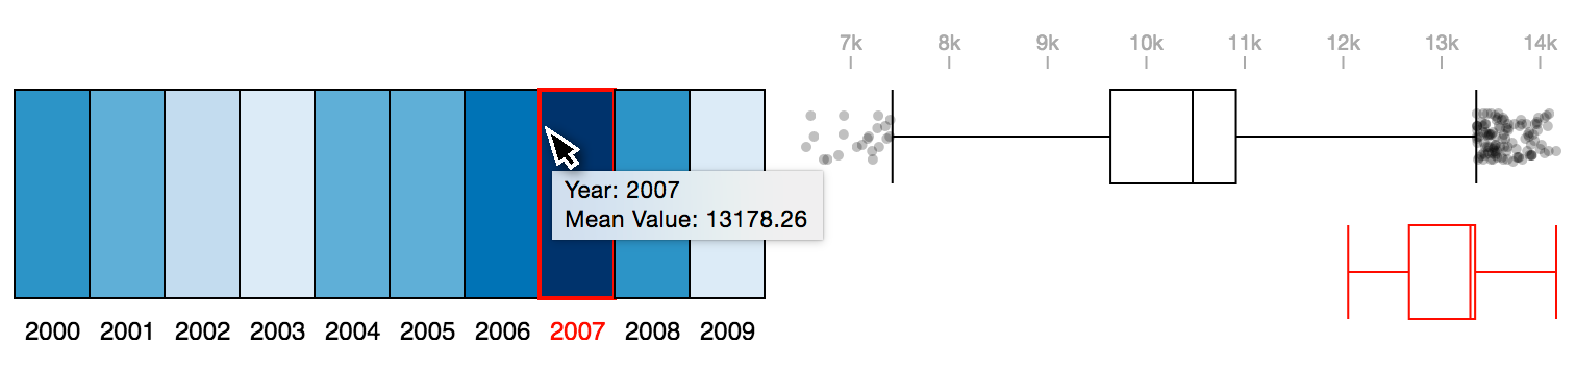
\includegraphics[width=0.975\textwidth]{figures/d3-boxplots.pdf}}
	\caption
	[
	    An interactive auxiliary boxplot prototype.
	]
	{
	    An interactive auxiliary boxplot prototype: boxplots corresponding to the brushed time period are shown alongside the boxplot for the entire time series.
	}
	\centering
	\label{emu:fig:interactive-boxplots}
\end{figure}

%-|-|-|-|-|-|-|-|-|-|-|-|-|-|-|-|-|-|-|-|-|-|-|-|-|-|-|-|-|-|-|-|-|-|-|-|-

\bstart{Juxtaposed stack and facets} Another reason to juxtapose views\index{view coordination!view juxtaposition} is to support fast alternation between tasks\index{task}.
Recall that the Drill Down ({\bf T2}) and Roll Up ({\bf T3}) tasks\index{task} are often performed in alternation, and we were concerned about the loss of context when switching between stacked bar charts\index{visual encoding!bar chart!stacked bar chart} or stacked area graphs\index{visual encoding!stacked area graph} and faceted\index{view coordination!faceting (small multiples)} bar charts\index{visual encoding!bar chart} or line graphs\index{visual encoding!line graph}.
To prevent this loss of context, we juxtaposed\index{view coordination!view juxtaposition} the stacked chart with the faceted\index{view coordination!faceting (small multiples)} charts, and provide linked highlighting between elements in the stack and those in the facets\index{view coordination!faceting (small multiples)}, as shown in \autoref{emu:fig:sandbox-stacks}; as a result, both the Drill Down and Roll Up tasks\index{task} are supported in a single display.
Currently, four facets\index{view coordination!faceting (small multiples)} are shown in a row, with additional facets\index{view coordination!faceting (small multiples)} wrapping to subsequent rows, sorted in the same order as the elements in the stack.

%-|-|-|-|-|-|-|-|-|-|-|-|-|-|-|-|-|-|-|-|-|-|-|-|-|-|-|-|-|-|-|-|-|-|-|-|-

\begin{figure}
	\centering
	\fbox{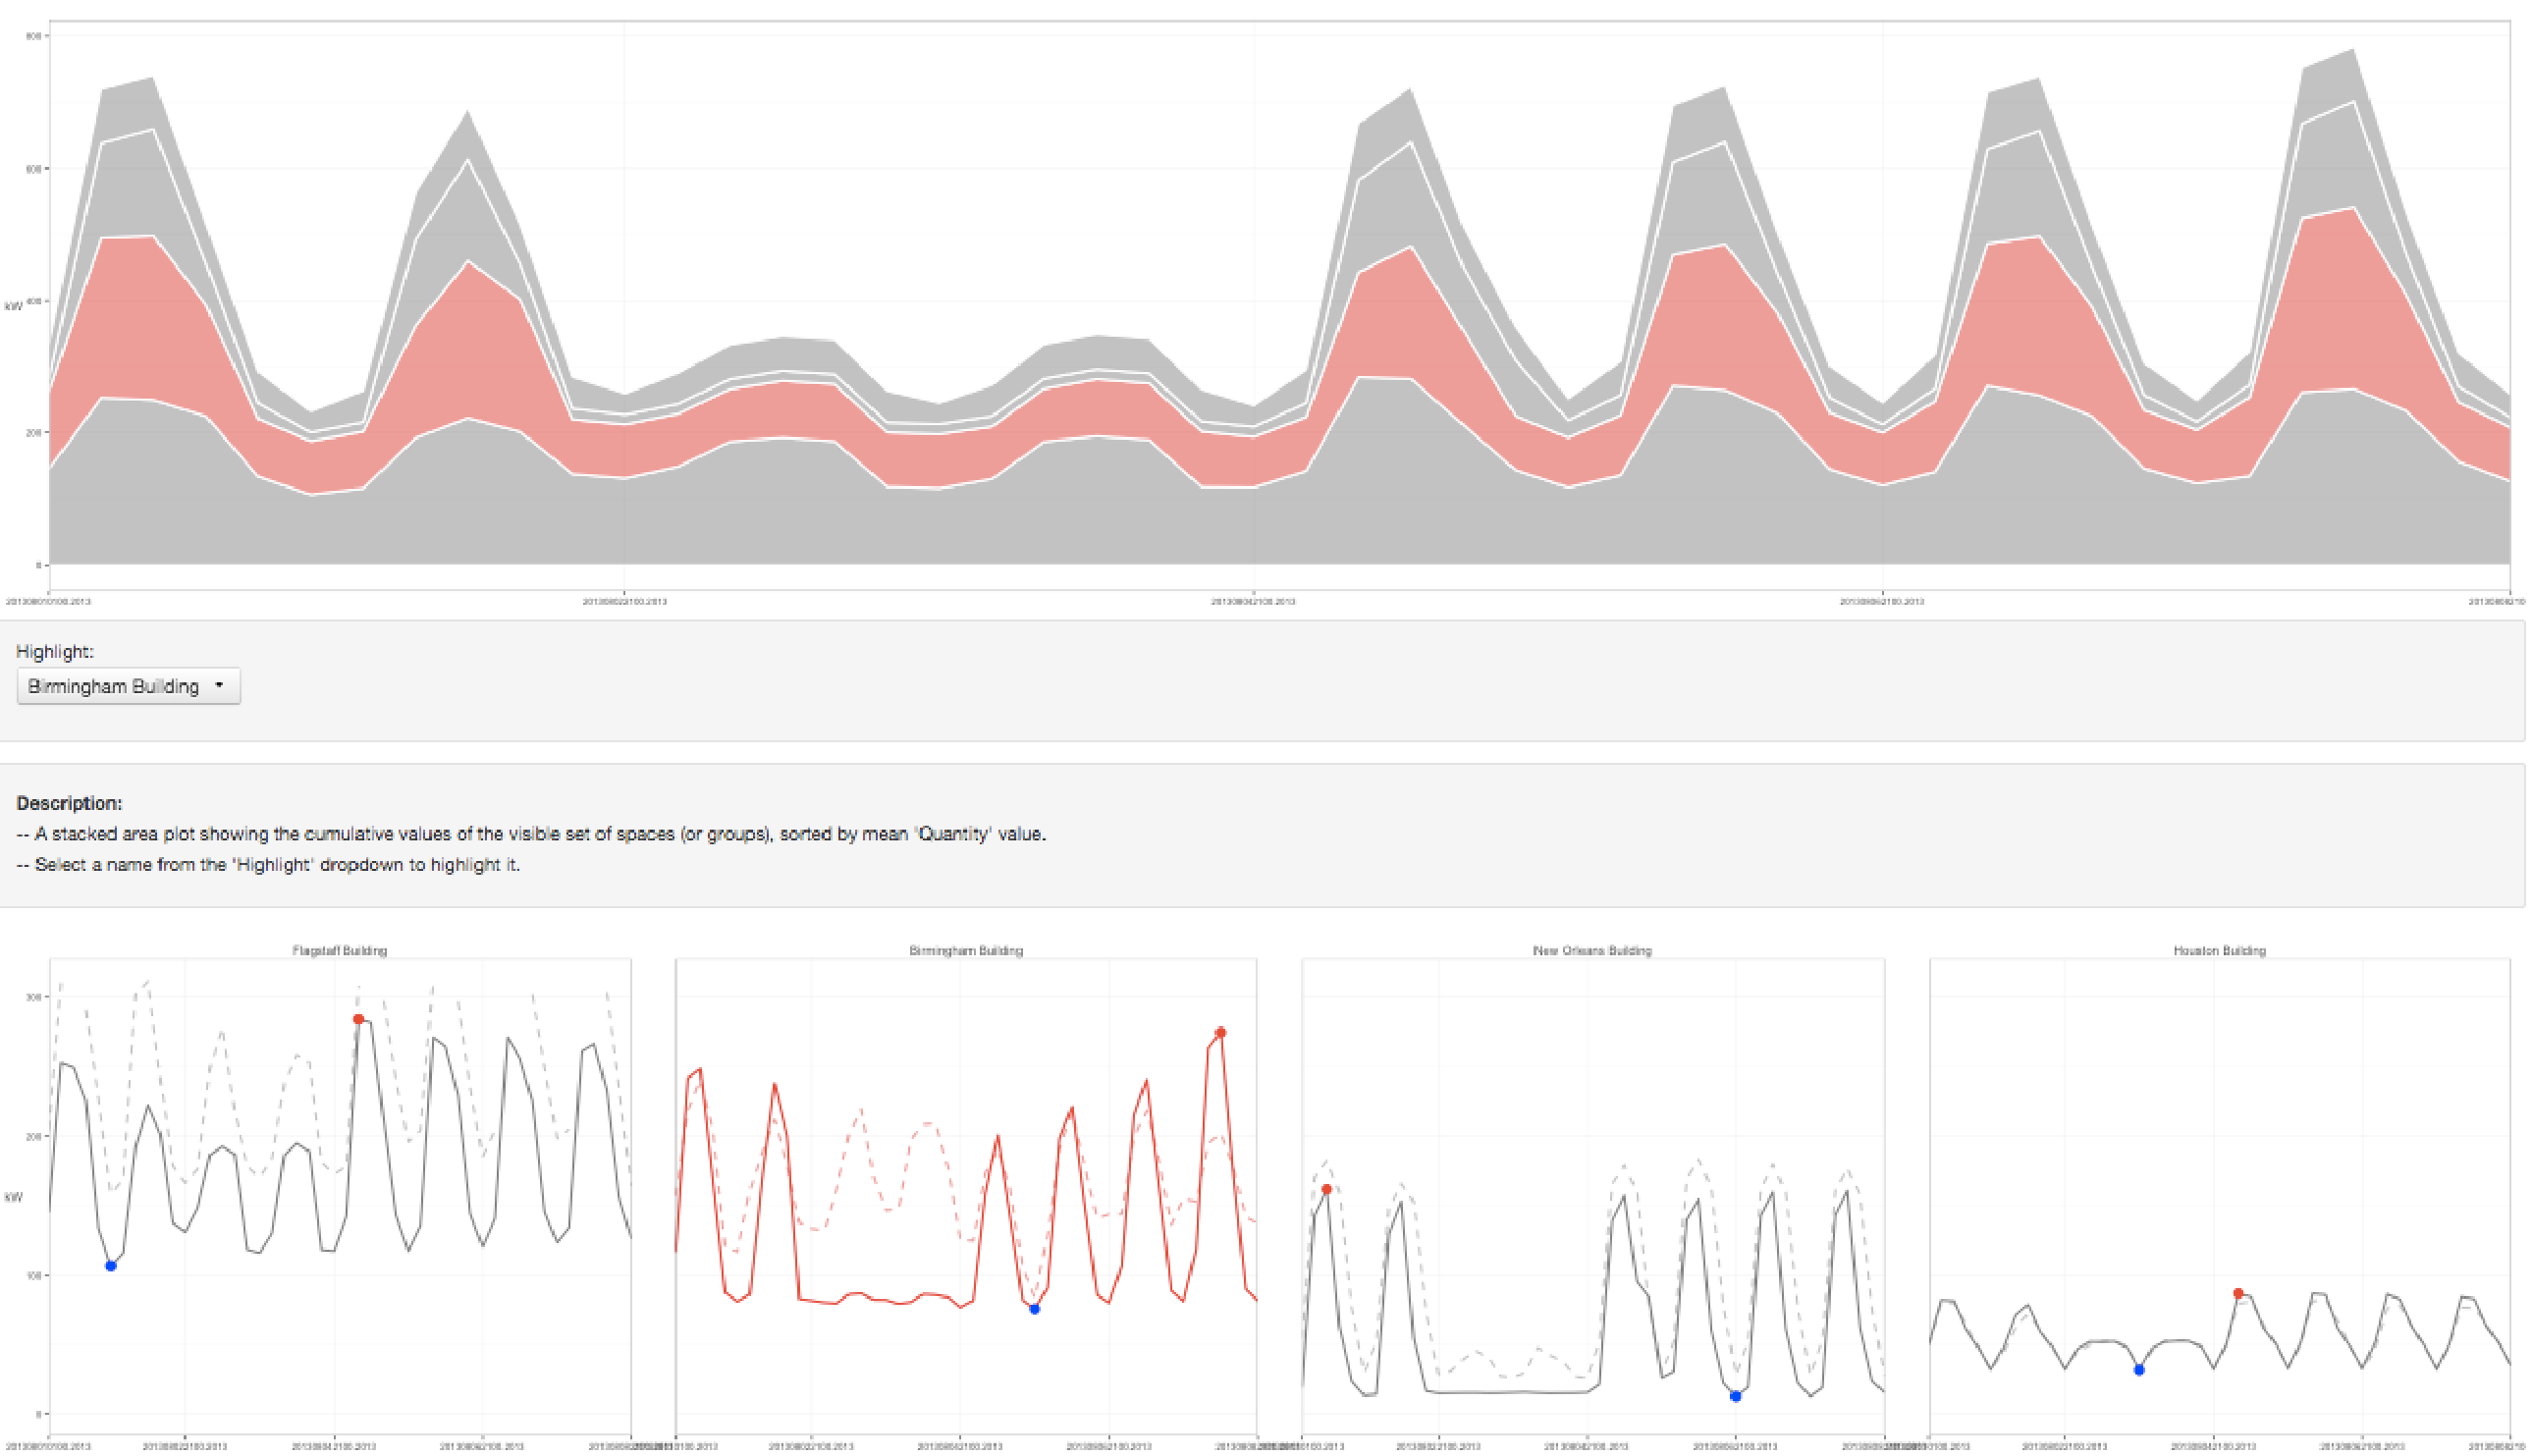
\includegraphics[width=0.975\textwidth]{figures/sandbox-stacks.pdf}}
	\caption
	[
	    A stacked area graph of \textsl{energy demand}.
	]
	{
	    A stacked area graph of \textsl{energy demand} data for four library buildings, juxtaposed alongside faceted line graphs of the same data. The same building is highlighted in red in both the stack and the facets.
	}
	\centering
	\label{emu:fig:sandbox-stacks}
\end{figure}

%-|-|-|-|-|-|-|-|-|-|-|-|-|-|-|-|-|-|-|-|-|-|-|-|-|-|-|-|-|-|-|-|-|-|-|-|-

\begin{sloppypar}
\bstart{Sequenced view navigation}
Recall that the Drill Down ({\bf T2}) and Roll Up ({\bf T3}) tasks\index{task} involve fewer buildings and finer temporal resolutions than the Overview ({\bf T1}) task\index{task}, which has a broader scope; 
thus, it would be inappropriate to juxtapose\index{view coordination!view juxtaposition} the Overview with the Drill Down and Roll Up views in a single display.
Instead, we considered how an energy analyst would {\tt navigate}\index{{\tt navigate}} between these views shown on separate displays\index{view coordination!view sequencing}.
Beginning with the matrix\index{visual encoding!matrix} and auxiliary boxplots\index{visual encoding!boxplots}, the energy analyst can perform the Overview task\index{task}, {\tt select}\index{{\tt select}} units of interest, and {\tt filter}\index{{\tt filter}} or {\tt aggregate}\index{{\tt aggregate}} buildings in the portfolio. 
If the currently selected\index{{\tt select}} unit of interest is {\it consumption} or {\it intensity}, {\tt selecting}\index{{\tt select}} a column of the matrix\index{visual encoding!matrix} directs the energy analyst to juxtaposed\index{view coordination!view juxtaposition} faceted\index{view coordination!faceting (small multiples)} and stacked bar charts\index{visual encoding!bar chart!stacked bar chart} that include every building from the matrix\index{visual encoding!matrix} and spanning the time period corresponding to the selected\index{{\tt select}} column. 
For {\it demand} data, the energy analyst is directed to faceted\index{view coordination!faceting (small multiples)} and stacked line graphs\index{visual encoding!line graph}.
At this point, the energy analyst can perform the Drill Down and Roll Up tasks\index{task} in alternation.
We demonstrate this multiple-view workflow\index{workflows} in a supplemental video\footnote{This video is available here: \url{http://cs.ubc.ca/labs/imager/tr/2015/MatchesMismatchesMethods/}}.
\end{sloppypar}

Finally, we also envisioned drilling down further to individual buildings. 
If the energy analyst {\tt selects}\index{{\tt select}} a cell or row of the matrix\index{visual encoding!matrix}, she will {\tt navigate}\index{{\tt navigate}} to a single bar or line graphs\index{visual encoding!line graph} for the corresponding building and time period.

%-------------------------------------------------------------------------
%-------------------------------------------------------------------------

\section{Results}
\label{emu:results}

%-------------------------------------------------------------------------
%-------------------------------------------------------------------------

We are pleased to report that our collaborators have adopted\index{adoption} a number of our designs into a new version of Energy Manager\index{Energy Manager}, shown in \autoref{emu:fig:emu}, which will soon be deployed to their large client base.
% Their client base is also expected to grow dramatically as a result of their recent partnership with a large utility company: tens of thousands of our collaborator's clients will now be able to analyze the energy performance of their building portfolios with the redesigned Energy Manager\index{Energy Manager}. 

%-|-|-|-|-|-|-|-|-|-|-|-|-|-|-|-|-|-|-|-|-|-|-|-|-|-|-|-|-|-|-|-|-|-|-|-|-

\begin{figure}
    \centering
	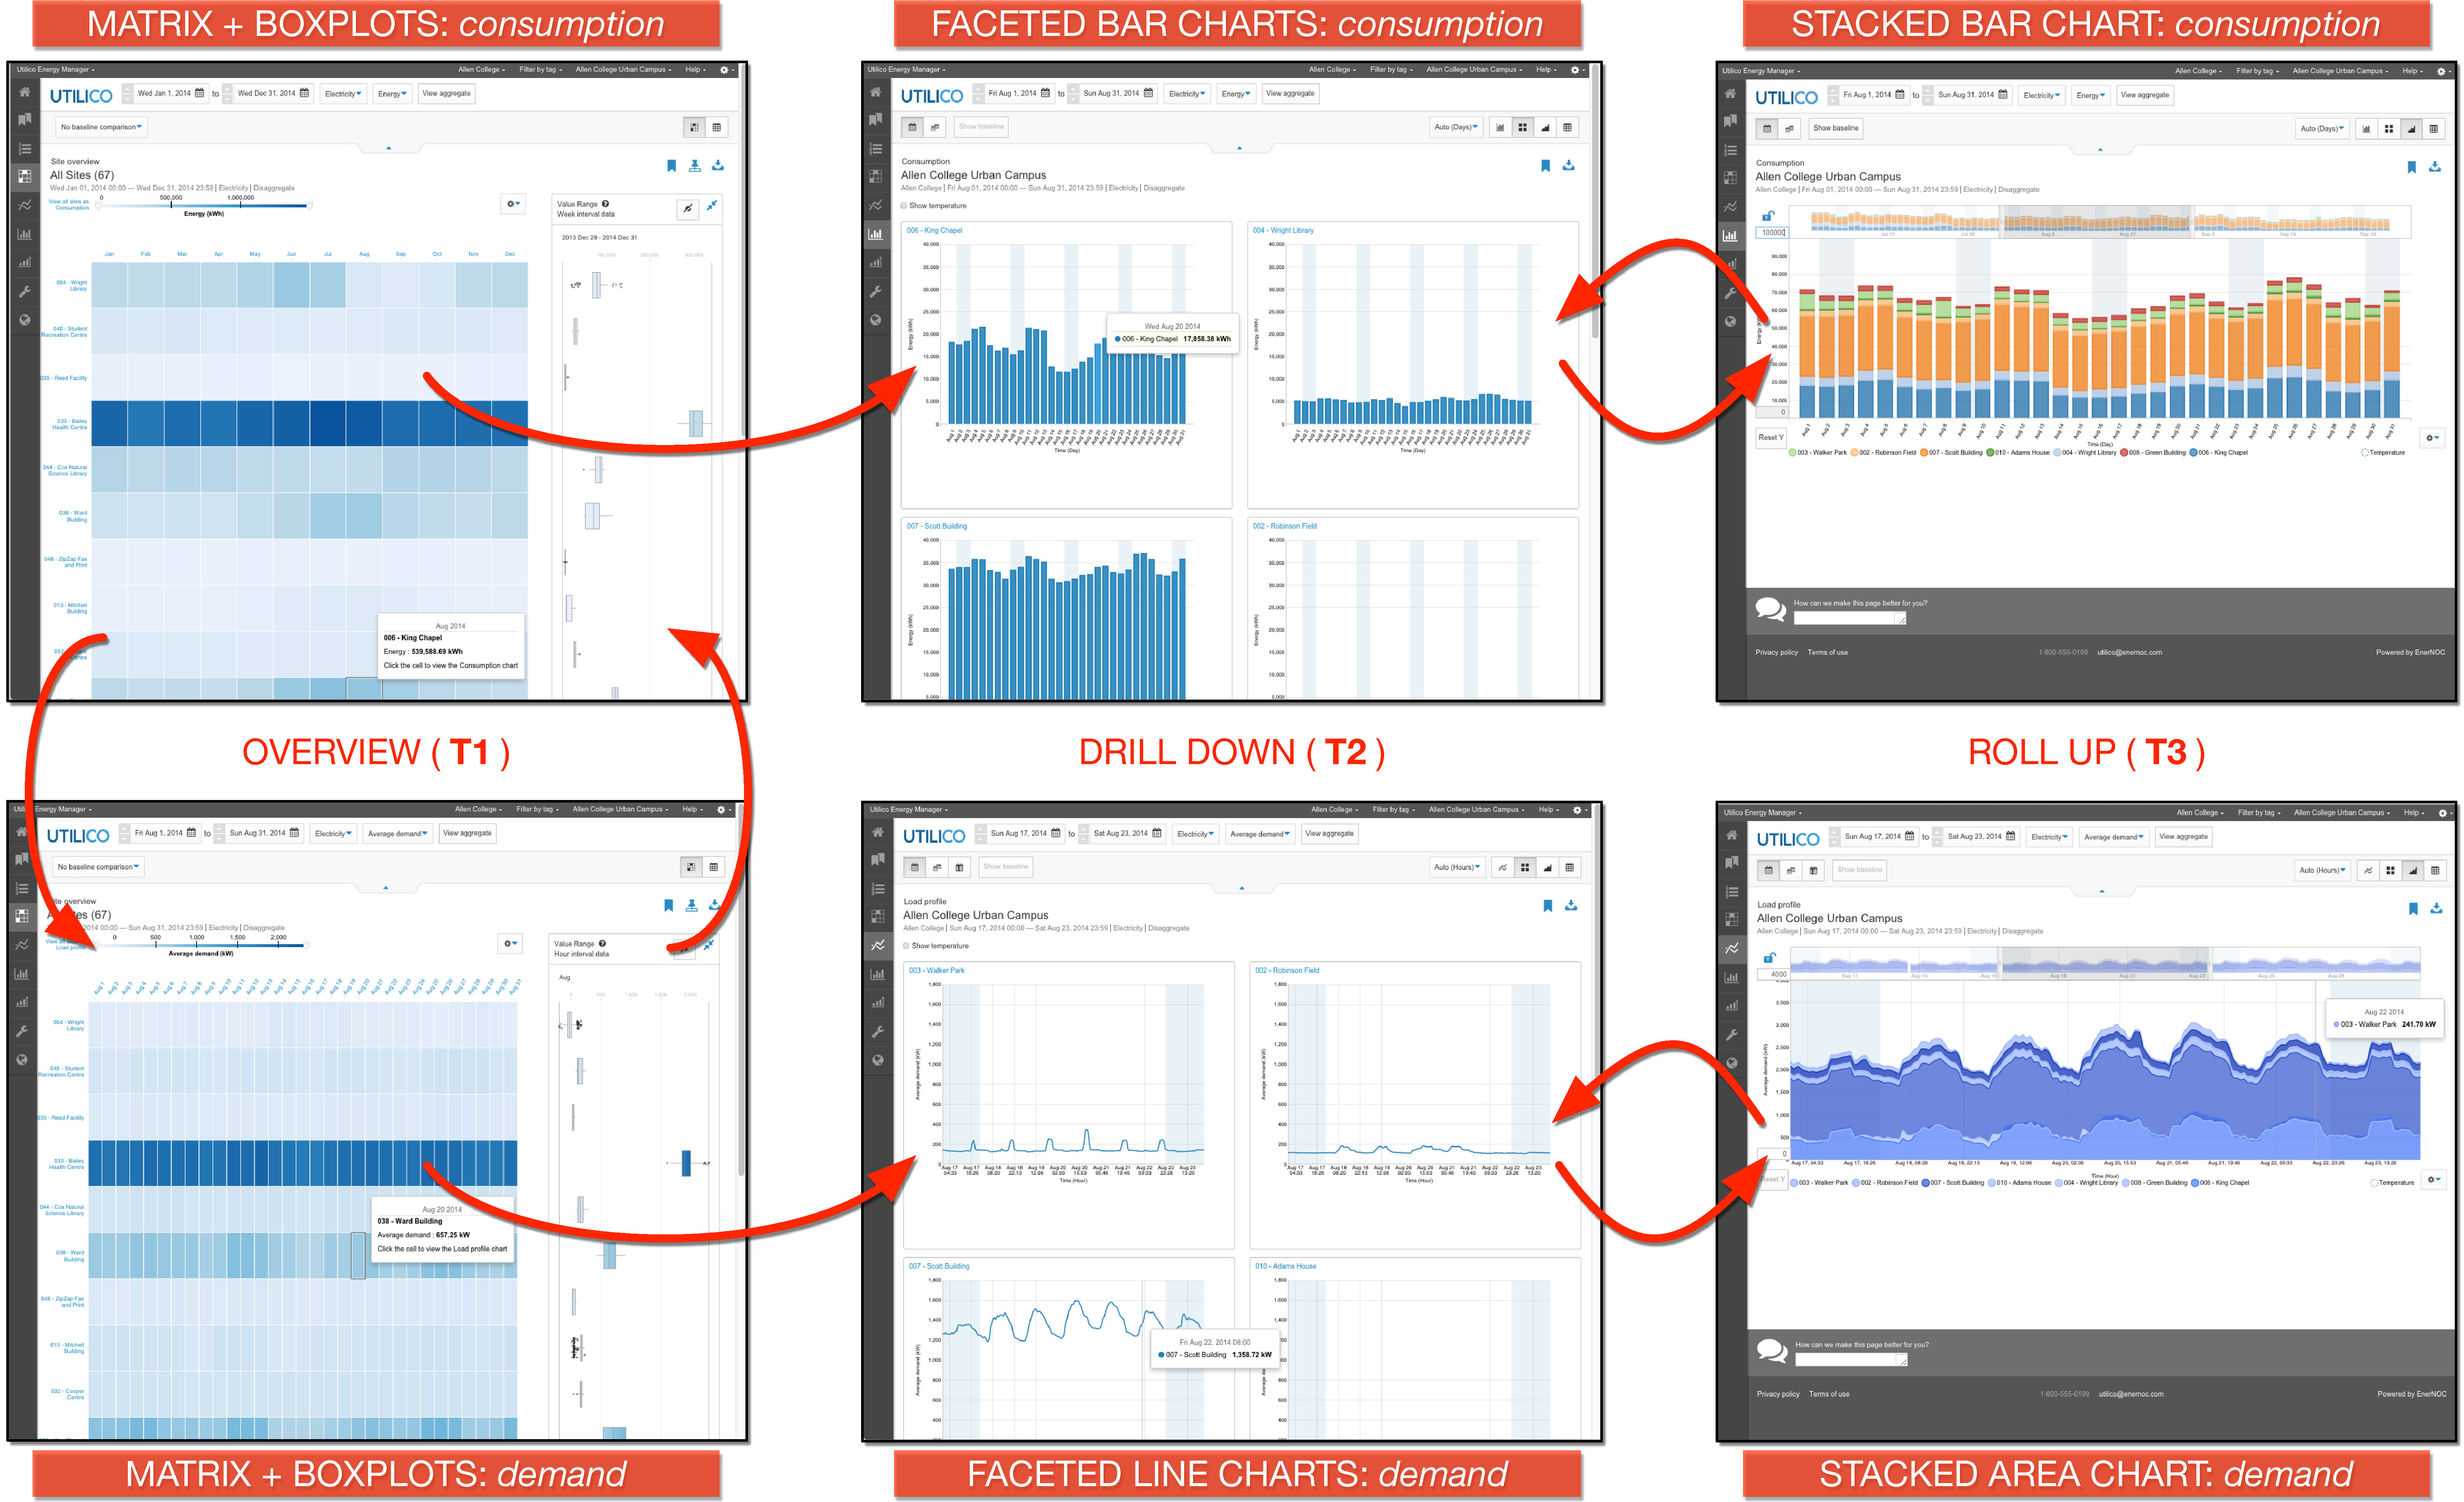
\includegraphics[width=\textwidth]{figures/emu.pdf}
	\caption
	[   
	    The redesigned Energy Manager that incorporates many aspects of our prototype designs.
	]
	{
	    The redesigned Energy Manager that incorporates many aspects of our prototype designs. On the left, the \textsl{Site Overview} (a time series matrix) is juxtaposed with coordinated \textsl{Value Range} (boxplot) views. An energy analyst can easily switch between units such as \textsl{energy consumption} or \textsl{energy demand} and {\tt filter} or {\tt aggregate} the set of buildings to those that share a common categorical tag; by {\tt selecting} a column of the matrix, she can drill down to faceted or stacked visual encodings of \textsl{consumption} (top middle, top right) or \textsl{demand} (bottom middle, bottom right).
	}
	\centering
	\label{emu:fig:emu}
\end{figure} 

%-|-|-|-|-|-|-|-|-|-|-|-|-|-|-|-|-|-|-|-|-|-|-|-|-|-|-|-|-|-|-|-|-|-|-|-|-

As in our sandbox environment, options for {\tt filtering}\index{{\tt filter}} and {\tt aggregating}\index{{\tt aggregate}} buildings according to shared categorical tags are now prominently and persistently shown in the menu at the top of the interface. 

The interface also provides the ability to {\tt select}\index{{\tt select}} units of interest and {\tt compare}\index{{\tt compare}} observed energy values against trusted historical values, as an alternative to comparing observed values to less trusted predicted values, overcoming a limitation of the original Energy Manager\index{Energy Manager}.

\bstart{Coordinated matrix and boxplots} a variant of our design described in \autoref{emu:design:workflows} has been incorporated into the redesigned Energy Manager\index{Energy Manager}.
The number of buildings shown depends on the window size, and more buildings appear as the energy analyst scrolls.
Our collaborators did consider the alternative calendar-based encoding\index{visual encoding!matrix!calendar (matrix)}, but ruled it out based on a requirement that arose late in the design process: that the redesigned Energy Manager\index{Energy Manager} be accessible on a tablet device. 
Partitioning the matrix\index{visual encoding!matrix} cells into calendars\index{visual encoding!matrix!calendar (matrix)} may result in calendar dates too small to be {\tt selectable}\index{{\tt select}} without zooming, which may incur a high implementation cost.
Meanwhile, the boxplots\index{visual encoding!boxplots} update when the energy analyst brushes\index{view coordination!brushing across views} the matrix\index{visual encoding!matrix} by hovering over a cell in the corresponding matrix\index{visual encoding!matrix} row, similar to the behaviour of the prototype we described in \autoref{emu:design:workflows}. 
Unlike our earlier prototype, a single boxplot\index{visual encoding!boxplots} is shown instead of showing one boxplot\index{visual encoding!boxplots} for the entire range and another boxplot\index{visual encoding!boxplots} for the brushed\index{view coordination!brushing across views} time period; when no time period in the matrix\index{visual encoding!matrix} is brushed\index{view coordination!brushing across views}, the boxplot\index{visual encoding!boxplots} for the entire time series\index{time-oriented data} is shown.

\bstart{Interactive workflows realized}\index{workflows} Another critical improvement over the original Energy Manager\index{Energy Manager} is the ability for an energy analyst to drill down from a row, column, or cell of the matrix\index{visual encoding!matrix} to stacked\index{visual encoding!stacked area graph}\index{visual encoding!bar chart!stacked bar chart}, faceted\index{view coordination!faceting (small multiples)}, superimposed\index{visual encoding!line graph!superimposed line graph}, or individual line graphs\index{visual encoding!line graph} and bar charts\index{visual encoding!bar chart}, as shown in \autoref{emu:fig:emu}.
The selected\index{{\tt select}} energy unit is retained across these transitions, so faceted\index{view coordination!faceting (small multiples)} line graphs\index{visual encoding!line graph} and stacked area graphs\index{visual encoding!stacked area graph} are used for {\it demand}, while faceted\index{view coordination!faceting (small multiples)} bar charts\index{visual encoding!bar chart} and stacked bar charts\index{visual encoding!bar chart!stacked bar chart} are used for {\it consumption}.
In faceted\index{view coordination!faceting (small multiples)} views\index{view coordination!faceting (small multiples)}, individual facets\index{view coordination!faceting (small multiples)} can be manually resorted via drag and drop.
Stacked and faceted\index{view coordination!faceting (small multiples)} views\index{view coordination!faceting (small multiples)} are currently shown separately; our collaborators are considering juxtaposing\index{view coordination!view juxtaposition} stacked and faceted views\index{view coordination!faceting (small multiples)}, such as in the design described in \autoref{emu:design:workflows}, which would allow for an uninterrupted alternation between the Drill Down ({\bf T2}) and Roll Up ({\bf T3}) tasks\index{task} in the same display.

%-------------------------------------------------------------------------
%-------------------------------------------------------------------------

\section{Discussion}
\label{emu:discussion}

%-------------------------------------------------------------------------
%-------------------------------------------------------------------------

\begin{sloppypar}
We now step back from specific aspects of visualization design for time-oriented data to discuss higher-level guidelines, to reflect upon on our methodology, and to indicate possible future work.
\end{sloppypar}

%-------------------------------------------------------------------------

\subsection{Guidelines: Familiarity and Trust}
\label{emu:discussion-guidelines}

%-------------------------------------------------------------------------

In addition to the specific guidelines regarding matches and mismatches between design choices and abstractions\index{task!task abstraction}\index{data abstraction} described in \autoref{emu:design:visenc}, we also propose guidelines relating to the themes of {\it familiarity}\index{familiarity} and {\it trust}.

\bstart{Familiarity}\index{familiarity} As with professionals in many other domains, energy analysts are accustomed to working predominantly with familiar\index{familiarity} visual encodings\index{visual encoding}, namely bars and lines.
When we introduced them to unfamiliar\index{familiarity} visual encodings\index{visual encoding}, we learned several things:

{\it Persevere despite unfamiliarity}\index{familiarity}: Though counter-intuitive, we learned that the juxtaposition\index{view coordination!view juxtaposition} of a matrix and a boxplot\index{visual encoding!boxplots}, two unfamiliar\index{familiarity} encodings, together with coordinated interaction\index{interaction} and highlighting, received more positive feedback than either of these encodings in isolation.
The issue of unfamiliarity\index{familiarity} with the time series\index{time-oriented data} matrix\index{visual encoding!matrix} was also partially resolved when we partitioned the cells into calendars\index{visual encoding!matrix!calendar (matrix)}.
We similarly persevered with the unfamiliar\index{familiarity} bump plot\index{visual encoding!bump plot}: by superimposing a layer of familiar\index{familiarity} bars on top of the bump plot\index{visual encoding!bump plot}, energy analysts were able to more easily interpret this rank-based visual encoding\index{visual encoding}.

{\it Beware assuming familiarity}\index{familiarity}: Introducing visual encoding\index{visual encoding} design choices using names that are well-known in the visualization literature can be misleading when they allude to familiar\index{familiarity} concepts in a way that is unfamiliar\index{familiarity} to the target audience, as we found with energy analysts and the term ``{\it heat map}''~\cite{Field2015,Wilkinson2009}\index{visual encoding!heat map}.
We initially referred to the time series\index{time-oriented data} matrices as ``heat maps''\index{visual encoding!heat map}, but this visualization term led to considerable confusion because of conflicting domain conventions\index{domain convention} with the energy-related meaning of {\it heat} and expectations raised by the word {\it map}: this encoding does not show energy solely used for heating, nor does it show the geographic location of buildings\footnote{This confusion is not unique to the energy domain~\cite{Field2015,Wilkinson2009}.}. 
In the redesigned Energy Manager\index{Energy Manager}, the time series\index{time-oriented data} matrix\index{visual encoding!matrix} is referred to as a {\it Site Overview}.

We also had a difficult experience gathering feedback about boxplots\index{visual encoding!boxplots} because the term itself was unfamiliar\index{familiarity}. 
In the redesigned Energy Manager\index{Energy Manager}, the boxplots\index{visual encoding!boxplots} are referred to as the {\it Value Range} chart, a term that appears to be understood. 
In hindsight, we could have explicitly solicited names for these views from energy analysts early on in the process based on their own descriptions~\cite{Metoyer2012}. 

\bstart{Trust} When a visualization technique or tool is used as part of the hypothesis generation and verification process, trust is imperative, especially for derived and aggregated values. 
Previous work has investigated the trustworthiness of visual encodings\index{visual encoding} for text-based data~\cite{Chuang2012}, and we now discuss the topic of trust motivated by our design of visual encodings\index{visual encoding} for time-oriented data\index{time-oriented data}.

{\it Auxiliary charts to combat information loss}: When the number of concurrent time series\index{time-oriented data} grows large, it is difficult and overwhelming to visualize individual values from each time series\index{time-oriented data}; instead, a common approach is to visualize derived aggregate values~\cite{McLachlan2008}.
This loss of detail is apparent in the original Energy Manager\index{Energy Manager}'s portfolio dashboard (\autoref{emu:fig:energy-manager-top}) as well as in the cells of our time series\index{time-oriented data} matrix\index{visual encoding!matrix} (\autoref{emu:fig:sandbox}).
Whenever there is a loss of detail, there is a loss of trust: one of the energy analysts remarked that these derived aggregate values hide information such as extreme values.
In juxtaposing\index{view coordination!view juxtaposition} the time series\index{time-oriented data} matrix\index{visual encoding!matrix} with auxiliary boxplots\index{visual encoding!boxplots} that update whenever a matrix\index{visual encoding!matrix} cell containing an aggregate value is brushed, we are not only restoring lost information: we are also restoring trust.

{\it Promote agency over derived values}: In our sandbox environment and in the redesigned Energy Manager\index{Energy Manager}, we provided explicit and obvious interactive controls for {\tt filtering}\index{{\tt filter}} and {\tt aggregation}\index{{\tt aggregate}}, as well as controls for unit {\tt selection}\index{{\tt select}} and normalization, controls that were missing in the original Energy Manager\index{Energy Manager}.
With these controls, we provide energy analysts agency over the creation of derived values and these values become more trusted.
Similarly, the redesigned Energy Manager\index{Energy Manager} includes the option to {\tt compare}\index{{\tt compare}} observed energy performance to selected\index{{\tt select}} historical values, as an alternative to {\tt comparing}\index{{\tt compare}} against predicted values generated by a ``black box'' statistical model; until there is some visual indication as to how the underlying model algorithms\index{algorithms} generate these values~\cite{Muhlbacher2014}, there will be little trust, and it is therefore preferable to provide the option to {\tt compare}\index{{\tt compare}} against trusted historical values.

%-------------------------------------------------------------------------

\subsection{Methodological Reflection}
\label{emu:discussion-methodology}

%-------------------------------------------------------------------------

Though our overall methodological approach is similar to many other visualization design studies~\cite{McKenna2014,Sedlmair2012}\index{design studies}, there are some specific aspects of our methodology that are unique to projects executed in company settings~\cite{Sedlmair2011}: we negotiated access to clients and to their portfolio data at the very beginning of our collaboration, and we encourage researchers considering similar collaborations to do the same.
In addition, we also engaged primarily with remote energy analysts, and our methodological decisions described in \autoref{emu:methodology} reflect this logistical difficulty~\cite{Brehmer2014a}.
We now take the opportunity to reflect on three other aspects of our methodology:

\bstart{Work domain analysis} {\it Worth it, and don't be daunted}. 
Conducting a rigorous and systematic work domain analysis\index{work domain analysis} can be time consuming and logistically challenging.
However, it is helpful to realize that authorities on work domain analysis~\cite{Vicente1999}\index{work domain analysis} established their methodologies in the design of high-risk, high-cost systems, such as nuclear power plant control rooms.
Work domain analysis\index{work domain analysis} and requirements analysis methodologies for many visualization design projects can be more flexible~\cite{McNamara2014} and creative~\cite{Goodwin2013} relative to those used for high-risk, high-cost systems.
A thorough work domain analysis\index{work domain analysis} need not take a year to complete, and subsequent phases of abstraction\index{task!task abstraction}\index{data abstraction} and iterative design can be carried out while continuing to develop an understanding of the work domain\index{work domain analysis}.

\bstart{Workflow prototyping}\index{workflows!workflow design} {\it A successful tool is more than a collection of views\index{view coordination}.}
In addition to using our sandbox environment to identify appropriate visual encodings\index{visual encoding} for individual tasks\index{task}, we also used it as a tool to generate possible {\it workflows}\index{workflows} that support a sequence of tasks\index{task!task sequence}.
Some visualization research projects stop before this step, but we argue for its importance.
We thought that confronting energy analysts with a combinatorial explosion of possibilities from a large set of visual encodings\index{visual encoding} and view parametrization options would fall short of a full solution to the problem at hand.

\bstart{Grounding design decisions} {\it Document everything, strive to be consistent and systematic}. 
One collaborator remarked that our approach often confirmed some earlier suspicions rather than introduced major surprises, where the novelty lay in a clear path to design decision-making that was missing before: {\it ``we performed an analysis of} [{\it Energy Manager's}] {\it flaws in a systematic way, put a name on them, and then tested with users''}\index{Energy Manager}. 
The exhaustive collecting and analyzing of qualitative data before and during design allowed us to justify the design decisions described in \autoref{emu:design:visenc} and \autoref{emu:design:workflows}. 
Presenting our consolidated findings and design justifications in concise and consistent annotated slide decks was highly appreciated by our collaborators.
Given this presentation of evidence, our collaborators adopted\index{adoption} our designs with confidence, much in the same way that the results of a controlled quantitative experiment can convince stakeholders~\cite{Sedlmair2011}. 

%-------------------------------------------------------------------------
%-------------------------------------------------------------------------

\section{Summary}
\label{emu:conclusion}

%-------------------------------------------------------------------------
%-------------------------------------------------------------------------

We conducted a design study\index{design studies} in the energy management\index{energy management} domain, one in which we collaborated with an energy analysis software company and their clients to develop a tool for analyzing the energy performance of large building portfolios.
We described visualization design choices framed in terms of {\it matches} and {\it mismatches} between abstractions\index{task!task abstraction}\index{data abstraction} and visual encoding\index{visual encoding} design choices that are transferable beyond the energy analysis domain, to other domains involve {\tt summarizing}\index{{\tt summarize}} and {\tt comparing}\index{{\tt compare}} many concurrent time series\index{time-oriented data}.
The matches include: 

\begin{itemize}
    \item Juxtaposed\index{view coordination!view juxtaposition} matrix\index{visual encoding!matrix} and boxplots\index{visual encoding!boxplots} for an Overview task\index{task}: {\tt lookup}\index{{\tt lookup}} and {\tt summarize}\index{{\tt summarize}} time-oriented quantitative data\index{time-oriented data} from all the items spanning a coarse period of time.
    \item Faceted\index{view coordination!faceting (small multiples)} bar charts\index{visual encoding!bar chart} and faceted\index{view coordination!faceting (small multiples)} line graphs\index{visual encoding!line graph} for a Drill Down task\index{task}: {\tt locate}\index{{\tt locate}} and {\tt compare}\index{{\tt compare}} time-oriented quantitative data\index{time-oriented data} for a group of items. 
    \item Stacked area graph\index{visual encoding!stacked area graph} and stacked bar charts\index{visual encoding!bar chart!stacked bar chart} for a Roll Up task\index{task}: {\tt explore}\index{{\tt explore}}, {\tt locate}\index{{\tt locate}}, and {\tt identify}\index{{\tt identify}} the proportion of a quantity associated with one item relative to the quantity associated with the item's group over time.
\end{itemize}

We also contributed seven lessons or guidelines pertaining to the themes of {\it familiarity}\index{familiarity} and {\it trust}, along with methodological guidance for visualization design studies\index{design studies}:

\begin{itemize}
    \item Familiarity\index{familiarity}: {\it Persevere despite unfamiliarity\index{familiarity}.}
    \item Familiarity\index{familiarity}: {\it Beware assuming familiarity\index{familiarity}.}
    \item Trust: {\it Auxiliary charts to combat information loss.}
    \item Trust: {\it Promote agency over derived values.}
    \item Work domain analysis\index{work domain analysis}: {\it Worth it, and don't be daunted.}
    \item Workflow prototyping\index{workflows!workflow design}: {\it A successful tool is more than a collection of views\index{view coordination}.}
    \item Grounding design decisions: {\it Document everything, strive to be consistent and systematic.}
\end{itemize}

As a result of our research and design process, our visualization designs were adopted\index{adoption} by our collaborator into their development of a redesigned commercial energy analysis application that will be deployed to client organizations.

%-------------------------------------------------------------------------
%-------------------------------------------------------------------------

\section{Addendum}
\label{emu:addendum}

\autoref{fig:emu:tasks}\footnote{\autoref{fig:emu:tasks} did not appear in our design study\index{design studies} paper~\cite{Brehmer2015}.} illustrates the three tasks\index{task} that we identified in \autoref{emu:task-abstractions}.

In \autoref{emu:task-abstractions}, we explicitly listed the {\tt actions}\index{{\tt actions}} and \underline{{\tt targets}}\index{{\tt targets}} involved in these three tasks\index{task}, and in \autoref{fig:emu:tasks}, \underline{{\tt targets}}\index{{\tt targets}} are depicted as the {\tt output}\index{{\tt output}} of each task\index{task}.
\autoref{fig:emu:tasks} also captures the sequential relationships between these tasks\index{task}, as well as the {\it how}\index{{\tt how}} perspective, indicating {\it how}\index{{\tt how}} the redesigned Energy Manager\index{Energy Manager} (shown in \autoref{emu:fig:emu}) supports these three tasks\index{task} in terms of design choices\footnote{This classification of {\it how} follows an extension to the typology by \citet{Munzner2014}, as illustrated in \autoref{fig:typology-vad-how}, rather than our original set of {\it how} design choices included in \autoref{typology:fig:typology}.}.

The Overview task\index{task} ({\bf T1}) is supported by two views\index{view coordination}: the data is {\tt encoded}\index{{\tt encode}} as a time series\index{time-oriented data} matrix\index{visual encoding!matrix} and as a series of boxplots\index{visual encoding!boxplots}, which are juxtaposed ({\tt arranged})\index{{\tt arrange}}\index{view coordination!view juxtaposition} in a single display.
The energy analyst can {\tt aggregate} all the buildings to view their combined consumption or demand, {\tt navigate}\index{{\tt navigate}} the list of buildings, {\tt navigate}\index{{\tt navigate}} the temporal range of the data, and finally {\tt select}\index{{\tt select}} data points in the time series\index{time-oriented data}, a brushing operation that updates the juxtaposed\index{view coordination!view juxtaposition} boxplots\index{visual encoding!boxplots}.

The Drill Down task\index{task} ({\bf T2}) is supported as follows: the energy analyst begins with the time series\index{time-oriented data} matrix\index{visual encoding!matrix} and boxplots\index{visual encoding!boxplots}, whereby she {\tt selects}\index{{\tt select}} or {\tt filters}\index{{\tt filter}} the set of buildings.
She is then directed to a new display, in which the data is {\tt encoded}\index{{\tt encode}} as a either a set of bar charts\index{visual encoding!bar chart} or line graphs\index{visual encoding!line graph} (depending on whether the data in question is consumption, intensity, or demand), which are juxtaposed ({\tt arranged})\index{{\tt arrange}}\index{view coordination!view juxtaposition} in a faceted\index{view coordination!faceting (small multiples)} small multiple layout.
She can then {\tt navigate}\index{{\tt navigate}} this set of buildings and {\tt navigate}\index{{\tt navigate}} the temporal range of the data.

Finally, the Roll Up task\index{task} ({\bf T3}) is supported by a single view in which the data for a group of buildings is {\tt encoded}\index{{\tt encode}} as stacked bar charts\index{visual encoding!bar chart!stacked bar chart} or stacked area graphs\index{visual encoding!stacked area graph} (again depending on whether the data in question is consumption, intensity, or demand).
With either of these charts, the energy analyst can {\tt navigate}\index{{\tt navigate}} the temporal range of the data and {\tt select}\index{{\tt select}} time points for individual buildings to view the specific values.

%-|-|-|-|-|-|-|-|-|-|-|-|-|-|-|-|-|-|-|-|-|-|-|-|-|-|-|-|-|-|-|-|-|-|-|-|-

 \begin{figure}
	\centering
	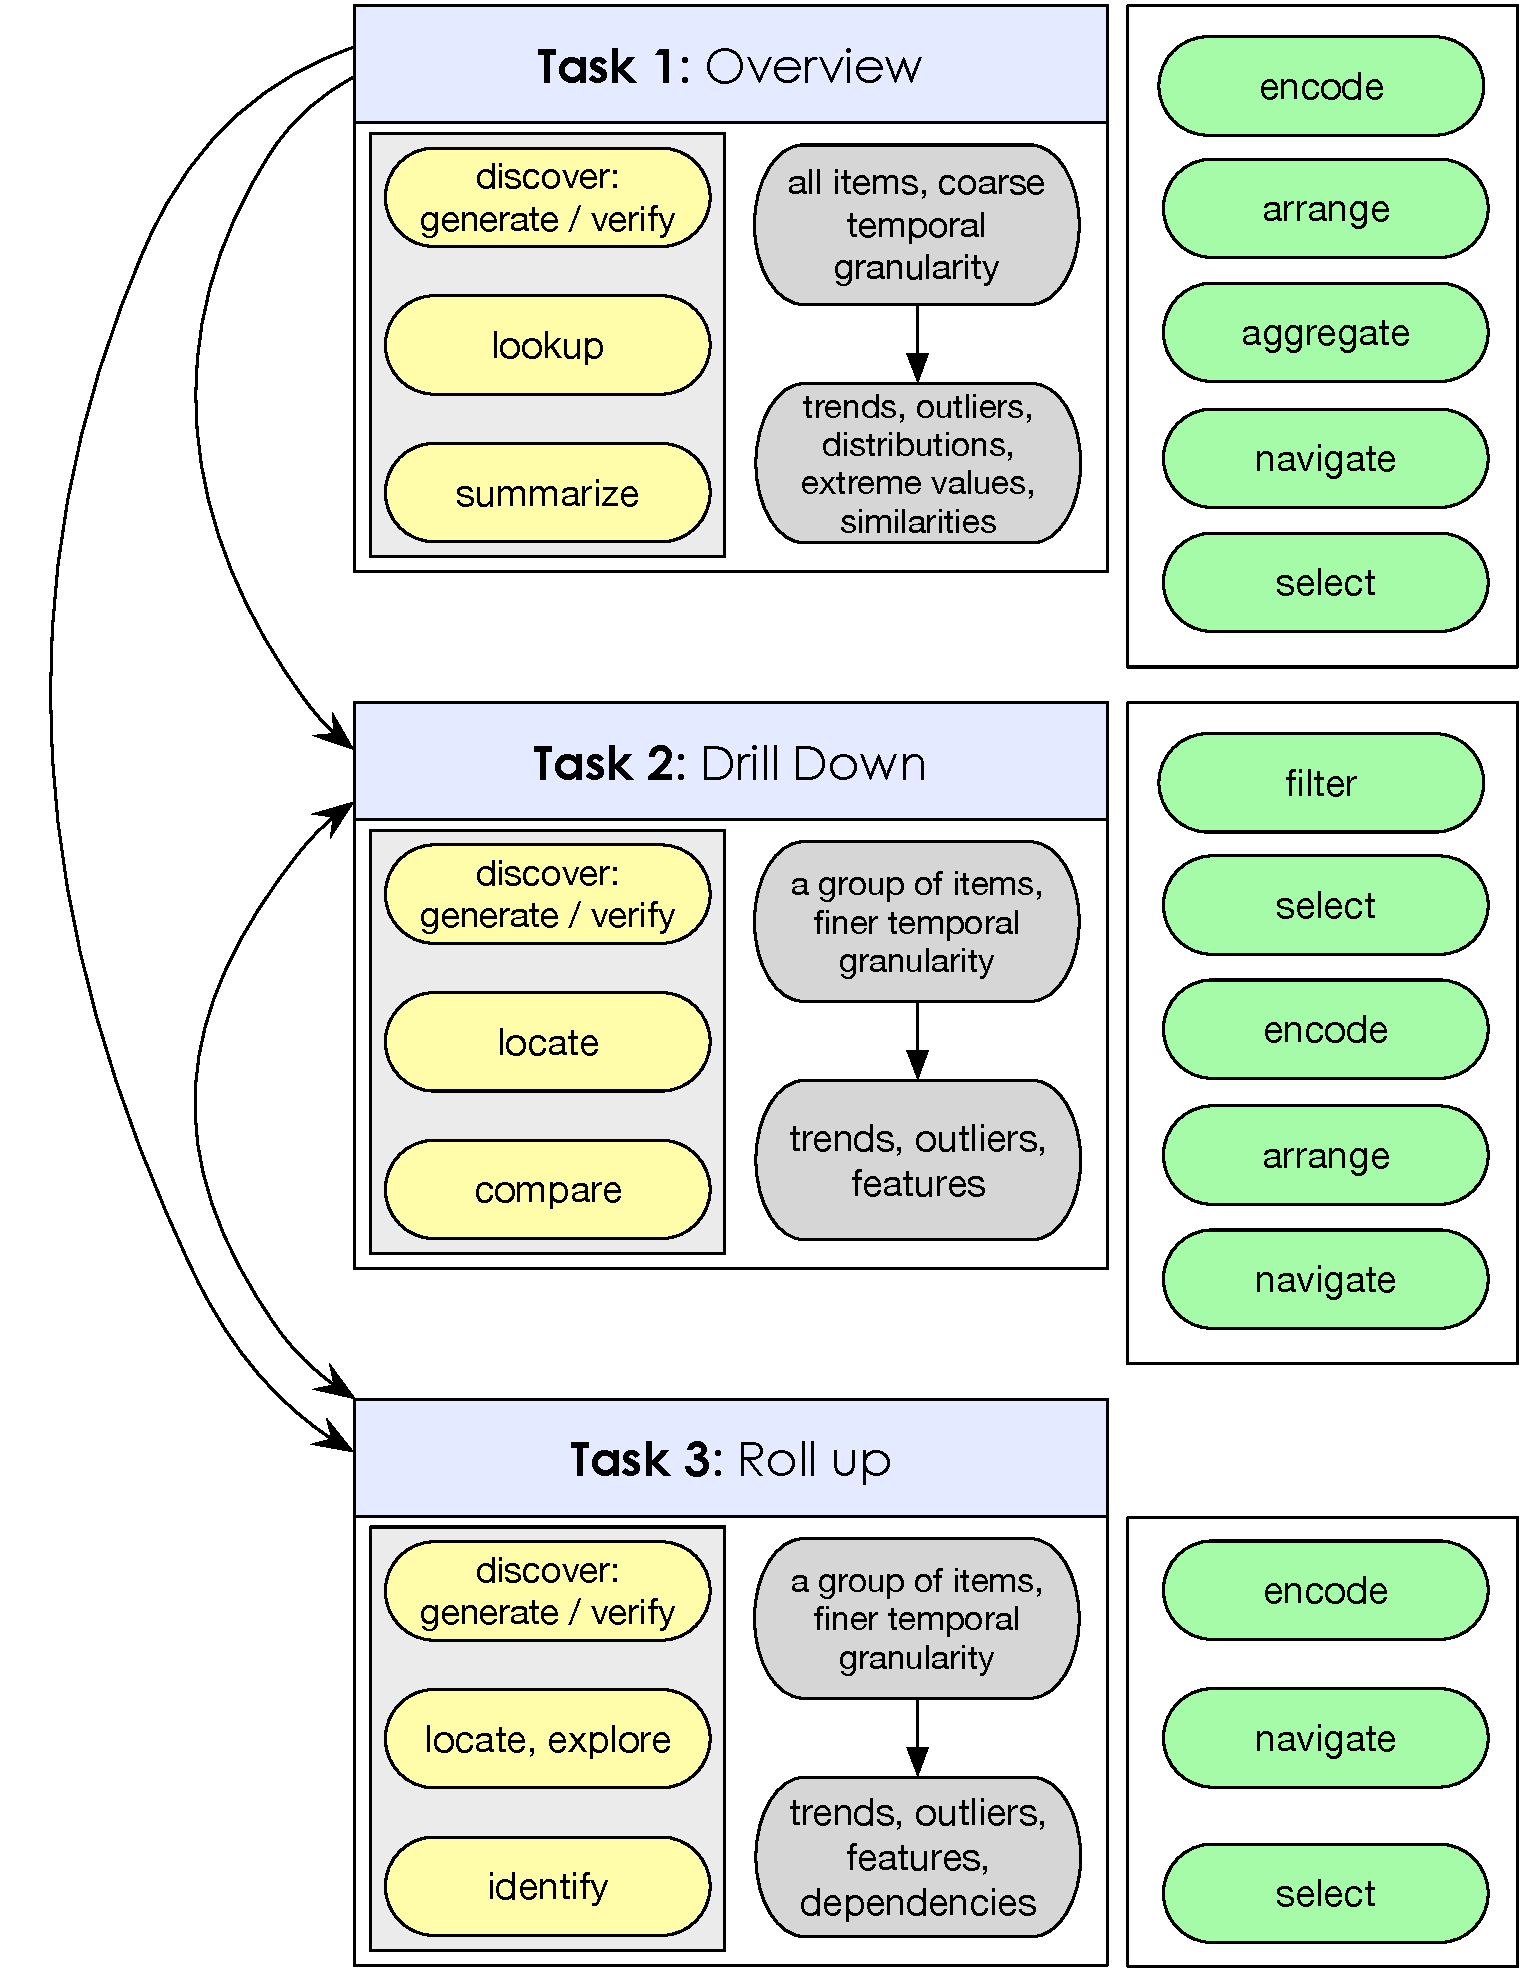
\includegraphics[width=0.95\textwidth]{figures/emu-tasks}
	\caption
	[
	   The three tasks identified in \autoref{emu:task-abstractions}.
	]
	{
	   The three tasks identified in \autoref{emu:task-abstractions}; colours correspond to the {\it why-what-how} structure of our task typology (see \autoref{typology:fig:typology}), where yellow is {\it why}, green is {\it how}, and grey is {\it what} defined in terms of {\tt inputs} and {\tt outputs}, where the {\tt outputs} are framed as {\tt targets}.
	   The classification of {\it how} corresponds to the redesigned Energy Manager as shown in \autoref{emu:fig:emu}.
	}
	\centering
	\label{fig:emu:tasks}
\end{figure}

%-|-|-|-|-|-|-|-|-|-|-|-|-|-|-|-|-|-|-|-|-|-|-|-|-|-|-|-|-|-|-|-|-|-|-|-|-

\endinput
